\chapter{Wobbling Motion in Nuclei}

The pioneering work of Bohr and Mottelson \cite{bohr1998nuclear} which was done more than 50 years ago lead to some interesting features regarding the collective phenomena in triaxial nuclei. Namely, they pointed out that a specific precessional motion of the nucleus's spin will take place when the rotational energy is sufficient. The angular momentum for triaxial nuclei is not aligned any of the principal axes of the ellipsoid, but it \emph{precesses} and \emph{wobbles} around one of these axes. They called this phenomenon \textbf{wobbling motion} (w.m.).
This combined motion comes from a consequence regarding the MOI. Indeed, the asymmetry of the three MOI makes the quantum mechanical nature of rotation to be possible around any of the three axes. As such, a \emph{main} rotation around the axis with the largest MOI will be the most energetically favorable, but the other two directions can \emph{quantum mechanically disturb} this main rotation, leading to this unique characteristic of triaxial nuclei.

The non-uniformity nature of w.m. was firstly studied for the `pure' rigid-rotators that correspond to the even-even nuclei. In this case, the w.m. can be treated as small amplitude oscillations of the total angular momentum $\mathbf{I}$ around the axis corresponding to the largest MOI.

\section{Wobbling Motion in Even-Even Nuclei}

The analytical expressions for wobbling excitations were firstly evaluated by Bohr and Mottelson using the so-called \emph{Harmonic Approximation} (HA). This can be described as a small-amplitude limit for the Triaxial Rigid Rotor Hamiltonian that was discussed in Chapter \ref{chapter4} (see Section \ref{trm-model}). In this limit, the projection of the total angular momentum onto the axis with largest MOI can be approximated $I_3\approx I$, meaning that the nucleus will do most of its rotation around this axis, with some `disturbance' from the other two principal of the triaxial rotor. 

For the description of this simple wobbler, one can consider the case when the $3$-axis has the largest MOI, and the following order holds true:
\begin{align}
    \mathcal{I}_3>\mathcal{I}_2>\mathcal{I}_1\ ,
\end{align}
or equivalently:
\begin{align}
    A_3<A_2<A_1\ .
\end{align}
The Hamiltonian can be written as:
\begin{align}
    \hat{H}_\text{rot}={\color{red}A_3I_3^2}+{\color{blue}\left(A_1I_1^2+A_2I_2^2\right)}
    \label{general-rotor-ham-evenA}
\end{align}

The different colors from Eq. \ref{general-rotor-ham-evenA} try to emphasize the fact that a Hamiltonian for the simple wobbler can be regarded as \emph{a main rotation around $3$-axis} (represented by red color) and \emph{the (precession + oscillation) of the total angular momentum} (represented by blue color).

The wobbling excitations which cause oscillations with small amplitudes for $\mathbf{I}$ about the $3$-axis are assumed to have a harmonic-like behavior, meaning that the final energy spectrum of a simple wobbler (even-even nucleus) will have the typical $\hbar\omega(n+1/2)$ behavior. Since this oscillator motion can be explained as `vibrations' of the total angular momentum around a steady position, where each wobbling excitation consists of an additional vibrating phonon, one can express the Hamiltonian in terms of \emph{boson} creation and annihilation operators. As such, the quantum mechanical treatment implies \cite{bohr1998nuclear}:
\begin{align}
    b^\dagger=\frac{1}{\sqrt{2I}}I_+\ ,\ b=\frac{1}{\sqrt{2I}}I_-\ ,\ \left[b,b^\dagger\right]\approx 1\ .
\end{align}

This initial quantization allows one to write Eq. \ref{general-rotor-ham-evenA} as a rotational term and a wobbling-specific one:
\begin{align}
    \hat{H}_\text{rot}&={\color{red}A_3I_3^2}+{\color{blue}H_w}\ ,\label{rot-ham-non-diagonal} \\
    {\color{blue}H_w}&={\color{blue}t_1\left(n+\frac{1}{2}\right)+\frac{1}{2}t_2(b^\dagger b^\dagger + bb)}\ ,
    \label{wob-ham-non-diagonal}
\end{align}
where the \emph{number of boson excitations} is denoted by $n$ and it is given by $n=b^\dagger b$. Each wobbling quanta will carry an angular momentum of one unit less with respect to the $3$-axis. The two factors $t_{1,2}$ are expressed in terms of the inertial parameters as \cite{bohr1998nuclear}:
\begin{align}
    t_1&=I(A_2+A_1-2A_3)\ , \\
    t_2&=I(A_2-A_1)\ .
\end{align}

Notice the linear dependence of the two parameters on the total angular momentum $I$. Moreover, depending on the values of $A_k$, the contribution of $t_{1,2}$ can be negative. Their behavior is shown within the right inset of Fig. \ref{fig-even-even-wobbling-energies}. Although the Hamiltonian $H_w$ is considered to have an oscillator-like behavior, its general expression does not look like a typical harmonic Hamiltonian. For this, the Hamiltonian given in Eq. \ref{wob-ham-non-diagonal} can be brought to a diagonalized form by introducing a new set of boson creation and annihilation operators. These operators will be written as linear combinations of $(b^\dagger,b)$:
\begin{align}
    c^\dagger=w_1b^\dagger-w_2b\ ,\\
    c=w_1b-w_2b^\dagger\ ,
\end{align}
where the two coefficients $w_{1,2}$ are defined in terms of $t_{1,2}$ as:
\begin{align}
    w_1&=\left[\frac{1}{2}\left(\frac{t_1}{\sqrt{t_1^2-t_2^2}}+1\right)\right]^{1/2}\ ,\nonumber\\
    w_2&=\left[\frac{1}{2}\left(\frac{t_1}{\sqrt{t_1^2-t_2^2}}-1\right)\right]^{1/2}\ .
    \label{eqs-w1-w2-terms-wobbling}
\end{align}

The terms $w_{1,2}$ verify the condition $w_1^2-w_2^2=1$ and they make the `dangerous' products ($b^\dagger b^\dagger$,$bb$) disappear in this new representation \cite{oi2006semi}. Note that there is no spin dependence inferred in Eq. \ref{eqs-w1-w2-terms-wobbling} such that $w_{1,2}$ are constant functions of spin, unlike the coefficients $t_{1,2}$. Moreover, introducing a number operator $\hat{n}=c^\dagger c$ and the excitation quanta $\hbar\omega_w$ defined as:
\begin{align}
    \hbar\omega_w=\sqrt{t_1^2-t_2^2}=2I\sqrt{(A_1-A_3)(A_2-A_3)}\ ,
    \label{wobbling-frequency-even-A}
\end{align}
then a final expression of $H_w$ can be expressed, which has a behavior typical to the \emph{harmonic oscillator}:
\begin{align}
    H_w=\hbar\omega_w\left(\hat{n}+\frac{1}{2}\right)\ .
    \label{wob-ham-diagonal}
\end{align}

In this expression, the excitation quanta $\hbar\omega_w$ which was defined in Eq. \ref{wobbling-frequency-even-A} in terms of $t_{1,2}$ is called \emph{wobbling frequency} and its increasing linearly with the total angular momentum. Accordingly, Eq. \ref{rot-ham-non-diagonal} can be re-written with the wobbling Hamiltonian defined in Eq. \ref{wob-ham-diagonal}:
\begin{align}
    \hat{H}_\text{rot}=A_3I(I+1)+\hbar\omega_w\left(\hat{n}+\frac{1}{2}\right)\ .
    \label{rot-wob-ham-diagonal}
\end{align}

Thus, in the HA, the eigenvalues of the rotor Hamiltonian can be expressed in terms of a \emph{wobbling phonon number} $n_w$ (which is the eigenvalue of the number operator $\hat{n}=c^\dagger c$) and a \emph{wobbling frequency} (defined in Eq. \ref{wobbling-frequency-even-A}):
\begin{align}
    E_{I,n}={\color{red}A_3I(I+1)}+{\color{blue}\hbar\omega_w\left(n_w+\frac{1}{2}\right)}\ .
    \label{eq-wobbling-energy-evenA}
\end{align}

The spectrum for an even-even wobbling nucleus is finally represented by Eq. \ref{eq-wobbling-energy-evenA}. Notice again the two colored terms that illustrate the energy coming from the rotation around the $3$-axis and the disturbed motion with small oscillations around the other two axes. Consequently, the wobbling character of the system will be generated by the latter harmonic term. The wobbling phonon number $n_w$ is related to the `strength' of the tilting for $\mathbf{I}$, indicating the fact that an increasing number for $n_w$ will result in oscillations with larger amplitudes around the other two axes. The phonon number takes only integer values $n_w=0,1,\dots$. In the inset $b)$ from Fig. \ref{wobbling-geometry-tilting-sketch}, a sketch which shows the tilting effect that the wobbling phonon number has on the total angular momentum vector is drawn. For completeness, the collective structure of two wobbling bands generated through phonon excitations is exemplified in inset $a)$ from Fig. \ref{wobbling-geometry-tilting-sketch}.

\begin{figure}
    \centering
    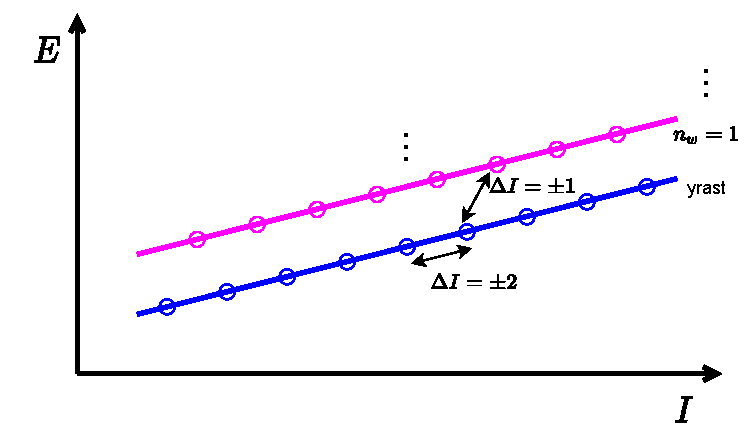
\includegraphics[scale=0.72]{Chapters/Figures/wobbling_n_schematic-1.pdf}
    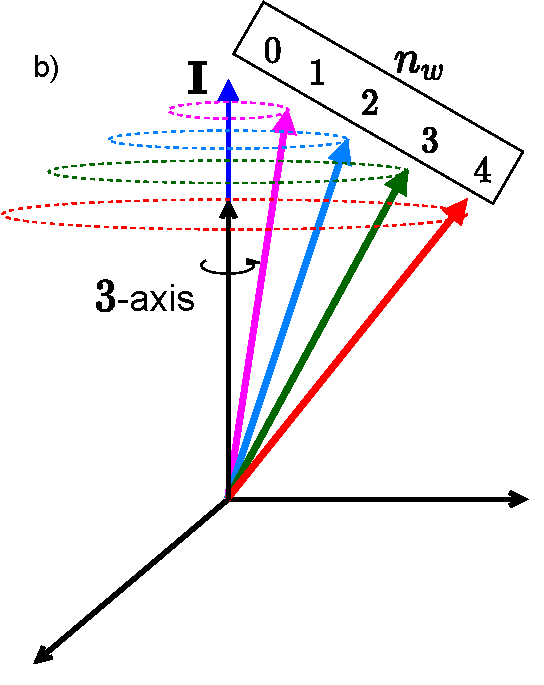
\includegraphics[scale=0.6]{Chapters/Figures/wobbling_n_schematic-2.pdf}
    \caption{\textbf{Left:} A typical wobbling structure for even-even nuclei. The yrast band contains even values of spins since the band has signature $\alpha=0$, while the first excited band has odd spins and $\alpha=1$. The intraband states differ by 2 units of angular momenta, while the interband ones differ with only one unit. \textbf{Right:} The increase of tilting angle between the rotational axis (the $3$-axis in this case) and the total angular momentum $\mathbf{I}$. With each wobbling phonon number, the total angular momentum tilts more and more, generating a `stronger' precessional motion (illustrated by the colored ellipses).}
    \label{wobbling-geometry-tilting-sketch}    
\end{figure}

An alternative way of depicting the wobbling term $H_w$ from Eq. \ref{wob-ham-non-diagonal} (or Eq. \ref{wob-ham-diagonal}) would be to express it more generally in terms of $I_1$ and $I_2$. When doing so, one achieves the following form (assuming that rotation is around the $3$-axis) \cite{oi2006semi}:
\begin{align}
    % H_w={\color{magenta}(A_1-A_3)I_1^2}+{\color{orange}(A_2-A_3)I_2^2}={\color{magenta}T_\text{kin}}+{\color{orange}T_\text{pot}}\ ,
    H_w=(A_1-A_3)I_1^2+(A_2-A_3)I_2^2=T_\text{kin}+T_\text{pot}\ ,
    \label{wobbling-hamiltonian-kin-pot-term}
\end{align}
where according to Ref. \cite{wen2015wobbling}, one can regard these two factors as a \emph{kinetic} and a \emph{potential} term. This way of expressing $H_w$ is instructive since it keeps a close contact with the `classical' picture of understanding the total energy of a system. An example with the behavior of $T_\text{kin}$ and $T_\text{pot}$ w.r.t. the first and second a.m. component, respectively, can be seen in Fig. \ref{kin-pot-wobbling-ham-example}.
\begin{figure}
    \centering
    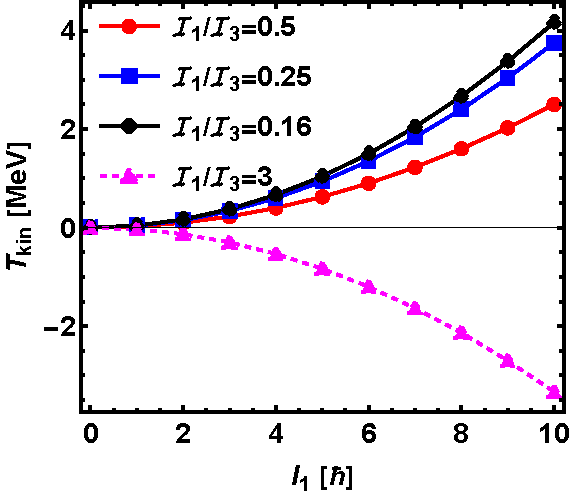
\includegraphics[width=0.49\textwidth]{Chapters/Figures/kin-pot-terms.pdf}
    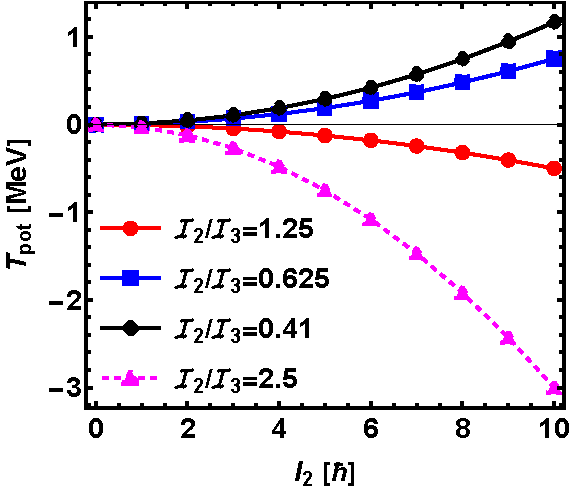
\includegraphics[width=0.49\textwidth]{Chapters/Figures/kin-pot-terms-2.pdf}
    \caption{The kinetic and potential terms from Eq. \ref{wobbling-hamiltonian-kin-pot-term} (which define the wobbling Hamiltonian) are graphically represented as function of $I_1$ and $I_2$, respectively. The a.m. components vary from $0$ to $10\hbar$. The MOI for each curve are as follow: $\mathcal{I}_1:\mathcal{I}_2:\mathcal{I}_3=10:25:20$ (red), $\mathcal{I}_1:\mathcal{I}_2:\mathcal{I}_3=10:25:40$ (blue), $\mathcal{I}_1:\mathcal{I}_2:\mathcal{I}_3=10:25:60$ (black), $\mathcal{I}_1:\mathcal{I}_2:\mathcal{I}_3=30:25:10$ (magenta). The unit for MOI is $\hbar^2\text{MeV}^{-1}$.}
    \label{kin-pot-wobbling-ham-example}
\end{figure}

As a quantitative analysis of the wobbling frequency and the rotor energy, one can take three arbitrary values for the moments of inertia (and, implicitly, the inertia factors $A_k$) and see the behavior of both $E_{I,n}$ and $\hbar\omega_w$ with increasing angular momentum and wobbling phonon number. Keep in mind that depending on the value of the wobbling phonon number, different spin sequences will be allowed. More precisely, from the invariance of the rotor w.r.t. rotations by $\pi$ about the principal axes for even-even nuclei, the signature quantum number $\alpha$ can take the values 0 and 1. Each wobbling band will have an alternating signature, starting with $\alpha=0$ for $n_w=0$ then $\alpha=1$ for $n_w=1$ and so on: even spin sequences appear for even values of $n_w$ and odd spin sequences appear for odd values of $n_w$ (see Fig. \ref{fig-even-even-wobbling-energies}).

The rotor energy from Eq. \ref{eq-wobbling-energy-evenA} is graphically represented for an arbitrary set of moments of inertia as a function of the nuclear angular momentum $I$ in the left inset of Fig. \ref{fig-even-even-wobbling-energies}. This pedagogical example contains rotational bands up to $n_w=5$ in the wobbling phonon number. From Fig. \ref{fig-even-even-wobbling-energies}, one can see the linear dependence on the total angular momentum for the wobbling frequency $\hbar\omega_w$ (the right inset) and the similar increasing trend of both the wobbling energy and frequency with respect to total spin.

\begin{figure}
    \centering
    % 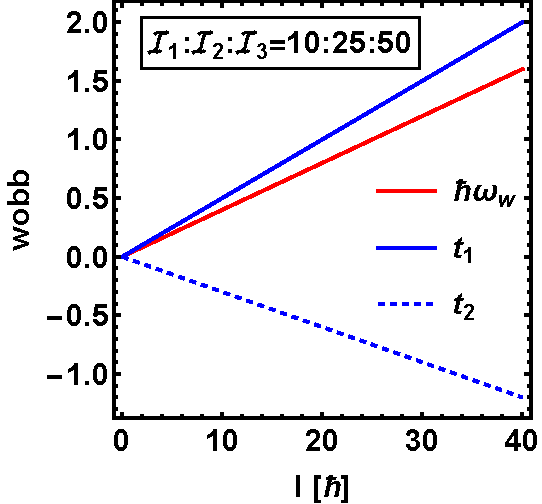
\includegraphics[scale=0.74]{Chapters/Figures/wobblingFreq-evenA.pdf}
    % 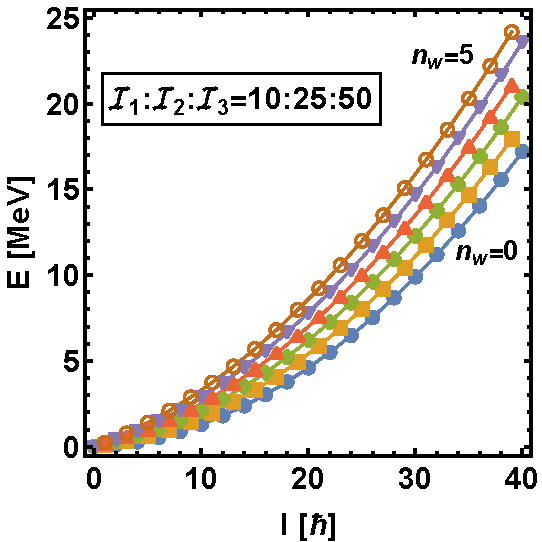
\includegraphics[scale=0.7]{Chapters/Figures/wobbling-evenA.pdf}
    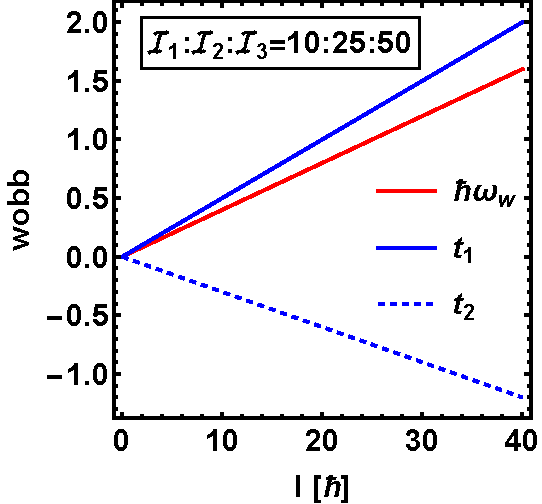
\includegraphics[scale=0.755]{Chapters/Figures/wobblingFreq-evenA.pdf}
    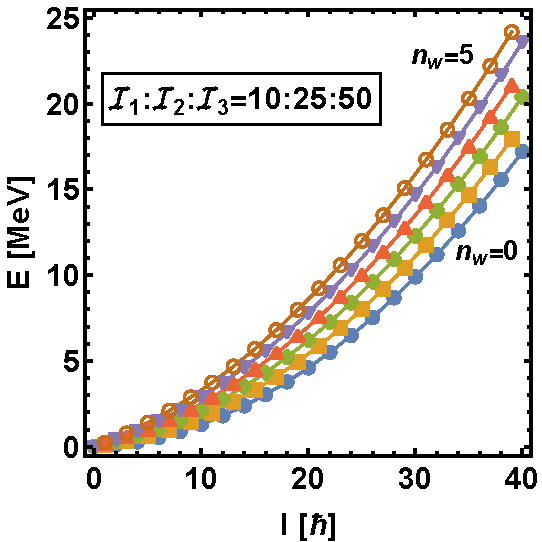
\includegraphics[width=0.49\textwidth]{Chapters/Figures/wobbling-evenA.pdf}
    \caption{\textbf{Left:} The energy spectrum for an even-even nucleus with three different moments of inertia, with the main rotation around the $3$-axis, according to Eq. \ref{eq-wobbling-energy-evenA}. Each wobbling band has alternating signature number $\alpha$ (starting with $\alpha=0$ for the ground state $n_w=0$ band). Notice the even/odd spin sequences for each band. \textbf{Right:}: The wobbling frequency (as given by Eq. \ref{wobbling-frequency-even-A}) plotted together with the linear terms $t_1$ and $t_2$ that are used to express $\hbar\omega_w$. Same set of MOI were used across both figures and the unit for $\mathcal{I}_i$ is $\hbar^2\ \text{MeV}^{-1}$.}
    \label{fig-even-even-wobbling-energies}
\end{figure}

Another instructive analysis would be the evolution of the components of $\mathbf{I}$ as functions of the polar and azimuthal angles $\theta,\varphi$. Indeed, expressing the three angular momentum components as:
\begin{align}
    I_1&=I'\sin\theta\cos\varphi\ ,\\
    I_2&=I'\sin\theta\sin\varphi\ ,\\
    I_3&=I'\cos\theta\ ,
    \label{angular-momentum-polar-components}
\end{align}
where $I'=\sqrt{I(I+1)}$, one can make a graphical representation for them, by letting $\theta$ and $\varphi$ vary within their corresponding intervals. In Fig. \ref{figs-angular-momentum-components-polar}, the quantities $I_1$ and $I_2$ are represented in the $(\theta,\varphi)$ plane for a fixed spin value $I=10\hbar$. Since the third component $I_3$ is independent of the azimuthal angle $\varphi$, it has been dismissed.

\begin{figure}
    \centering
    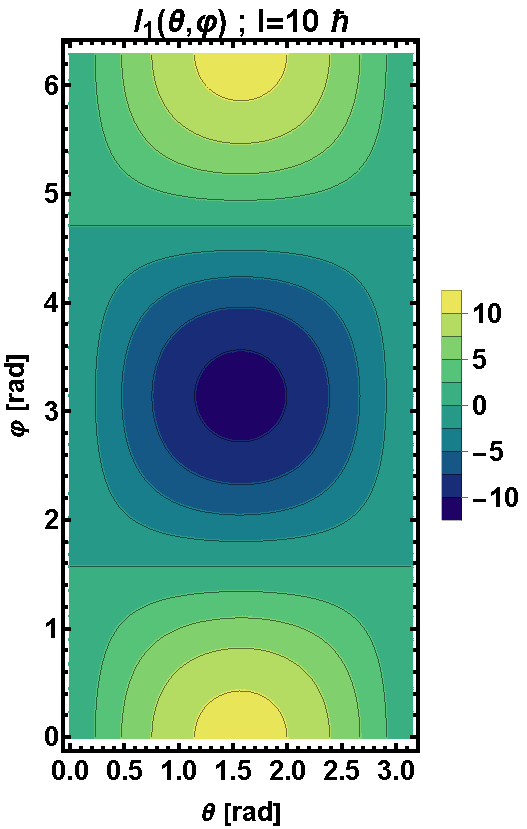
\includegraphics[scale=0.66]{Chapters/Figures/angular_components-TRM-1.pdf}
    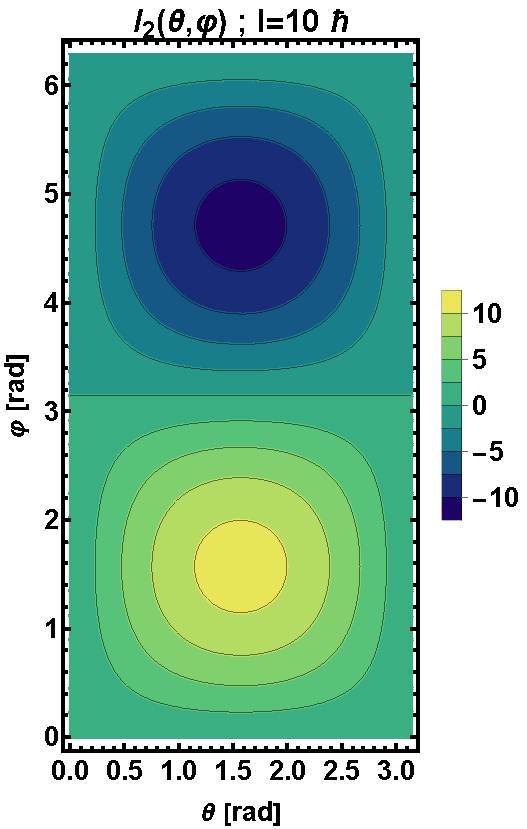
\includegraphics[scale=0.66]{Chapters/Figures/angular_components-TRM-2.pdf}
    \caption{The geometrical representation of the first and second component of the total angular momentum $\mathbf{I}$ as functions of the polar angles, according to Eq. \ref{angular-momentum-polar-components}.}
    \label{figs-angular-momentum-components-polar}
\end{figure}

The other relevant observables that can be calculated for simple wobbler within the HA are the two quadrupole moments $Q_{20,22}$ and the intraband + interband $B(E2)$ transition probabilities. The quadrupole components are expressed in terms of the intrinsic quadrupole moment $Q_0$ and the triaxiality parameter as \cite{shoji2006microscopic}:
\begin{align}
    Q_{20}=Q_0\cos\gamma\ ,\ Q_{22}=\frac{1}{\sqrt{2}}Q_0\sin\gamma\ .
    \label{quadrupole-components-q20-q22}
\end{align}

These components can be furthermore used to determine the intraband $B(E2)$ transition probabilities \cite{wen2015wobbling}:
\begin{align}
    B(E2;(n,I)\to(n,I-2))=\frac{5}{16\pi}Q_{22}^2\ ,
    \label{intraband-probability-simple-wobbler}
\end{align}
and also the interband transitions:
\begin{align}
    B(E2;(n,I)\to(n-1,I-1))&=\frac{5}{16\pi}\frac{n}{I}\left(\sqrt{3}Q_{20}w_1+\sqrt{2}Q_{22}w_2\right)^2\ , \label{interband-probability-simple-wobbler-1}\\
    B(E2;(n,I)\to(n+1,I-1))&=\frac{5}{16\pi}\frac{n+1}{I}\left(\sqrt{3}Q_{20}w_2+\sqrt{2}Q_{22}w_1\right)^2\ .
    \label{interband-probability-simple-wobbler-2}
\end{align}

Notice that for the intraband transitions, going from the state $I$ to $I-2$ will only depend on the quadrupole component $Q_{22}$ squared (Eq. \ref{quadrupole-components-q20-q22}), thus making the transitions spin-independent.

\subsubsection*{Triaxial rotor energy vs. wobbling energy}

An important discussion should be made regarding the nomenclature for energies when referring to wobbling motion. As shown in Eq. \ref{eq-wobbling-energy-evenA}, the energy spectrum for a simple wobbler can be determined for every phonon number and spin sequences. However, that is the `full' spectrum  of the wobbler, which is composed of the \emph{yrast} states with $n_w=0$ and the \emph{excited states} having $n_w=1,\dots$ and so on. On the other hand, the so-called \emph{wobbling energies} are defined in terms of these `absolute values' (i.e., $E_{I,n}$) with the following rules \cite{wen2015wobbling}:
\begin{align}
    E_\text{wob}(I_\text{even})&=E_{I,n}-E_{I,0}\ , \label{eq-wobbling-energy-definition-evenA} \\
    % E_\text{wob}(I_\text{even})&=E_{I,n}-E_{I,0}\ ,\nonumber \\
    E_\text{wob}(I_\text{odd})&=E_{I,n}-\frac{1}{2}\left(E_{I-1,0}+E_{I+1,0}\right)\ ,
    \label{eq-wobbling-energy-definition-oddA}
\end{align}
where the former wobbling energy corresponds to the even values of $I$ and the latter is applied for odd values of $I$. Very often within literature the energies calculated via Eq. \ref{eq-wobbling-energy-evenA} are referred to also as wobbling energies, which is not the same as Eq. \ref{eq-wobbling-energy-definition-oddA}, so a distinction should be made clear.

\subsection{Testing the Harmonic Approximation}
\label{ba-130-numerical-calculations}

It is worth going further and apply the HA formalism for even-even nuclei for an existing spectrum. As such, one can take $^{130}$Ba as a testing example. As it will be discussed in a follow-up section, it turns out that experimental observations for wobbling structures in even-mass isotopes have been very scarce. Nevertheless, very recently, Petrache et al. identified a large collection of band structures in $^{130}$Ba \cite{petrache2019diversity}. Two of them are reported to be of wobbling nature \cite{chen2019transverse}. Having these two collective bands, one can check if the energy formula given in Eq. \ref{eq-wobbling-energy-evenA} for the simple wobbler can be applied for this isotope.

The method described in here will be based on a \emph{fitting procedure}, namely a set of parameters will be extracted from the expression of $E_{I,n}$ and they will be adjusted such that the experimental data is best reproduced by the theoretical model. This kind of approach works really well for `well-behaved' model functions and if the input data is large enough to reach a good fit precision. More often than not, if the model function contains parameters which have a clear physical meaning, then fitting becomes a suitable approach. In fact, in the following chapters, the developed formalism will verify the experimental data through similar fitting procedures (although their `core'-implementation will be more complex).

Looking at the energy formula from Eq. \ref{eq-wobbling-energy-evenA}, at a first glance, two fitting parameters would appear, namely the largest moment of inertia $\mathcal{I}_3$ and the wobbling frequency $\hbar\omega$. However, the wobbling frequency is furthermore dependent on the other two moments of inertia (as per Eq. \ref{wobbling-frequency-even-A}), meaning that one can use the set $\mathcal{P}_\text{fit}=\left[\mathcal{I}_1,\mathcal{I}_2,\mathcal{I}_3\right]$ as appropriate fitting parameters. The wobbling phonon number $n_w$ is attributed as follows: $n_w=0$ for the yrast band (denoted throughout calculations with B1) and $n_w=1$ for the first excited band (denoted with B2). The band B1 has signature $\alpha=0$ so it is the even-spin sequence, while B2 has odd spins. The experimental data regarding spins and energies for the two bands correspond to the measurements done in Ref. \cite{petrache2019diversity}.

\subsubsection{Energy Spectrum}

Indeed, by following the procedure described above, the set $\mathcal{P}_\text{fit}$ is obtained. The parameters, i.e., the three moments of inertia are shown in Table \ref{table-params-ba130}. Remarking the fact that the largest MOI which was obtained via the fitting procedure is the one corresponding to the $3$-axis. With these parameters, the theoretical energies are determined numerically and the two bands are compared to the measured data in Fig. \ref{plot-ba130-excitation-energies}. Concerning the fitted energies, in the present calculations, instead of working with the `absolute energies' (i.e., the exact values of the energies that correspond to the measured spectrum), the \emph{excitation energies} were used instead \cite{raduta2017semiclassical,raduta2018wobbling,raduta2020towards}. These are determined by subtracting the band-head energy of B1 (the $10^+$ level) from each excited state of B1 and B2. By doing this, the accuracy of the results will be improved. The excitation energy for a spin state $I$ is given as:
\begin{align}
    E(I)=E_\text{abs}(I)-E_\text{abs}(I_0)\ ,
    \label{excitation-energy-general-formula}
\end{align}
where `abs.' signifies the absolute value for $E$ at that particular spin state ($I\geq I_0$) and $I_0$ is the band-head state within the yrast band.

\begin{table}
    \centering
    \resizebox{0.35\textwidth}{!}{%
    \begin{tabular}{|cccc|}
    \hline
    \multicolumn{4}{|c|}{$\mathcal{P}_\text{fit}$}                                                                                                                        \\ \hline
    \multicolumn{1}{|c|}{$\mathcal{I}_1$} & \multicolumn{1}{c|}{$\mathcal{I}_3$} & \multicolumn{1}{c|}{$\mathcal{I}_2$} & \multicolumn{1}{c|}{Unit}                     \\ \hline
    \multicolumn{1}{|c|}{27}                & \multicolumn{1}{c|}{22}                & \multicolumn{1}{c|}{43}                & \multicolumn{1}{c|}{$\hbar^2\text{MeV}^{-1}$} \\ \hline
    \end{tabular}%
    }
    \caption{The parameter set $\mathcal{P}_\text{fit}$ obtained from the fitting procedure of the excitation energies of the two wobbling bands (B1 and B2) for $^{130}$Ba. The model function corresponds to the energy of a simple wobbler (see Eq. \ref{eq-wobbling-energy-evenA}).}
    \label{table-params-ba130}
\end{table}

\begin{figure}
    \centering
    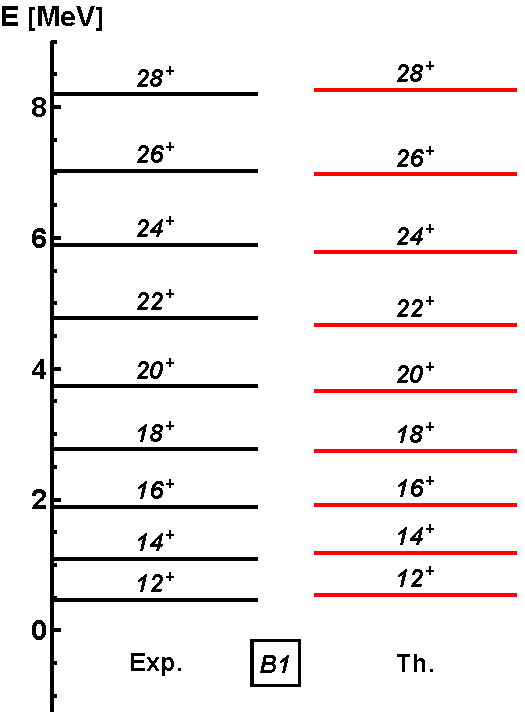
\includegraphics[width=0.46\textwidth]{Chapters/Figures/ba130-band1.pdf}
    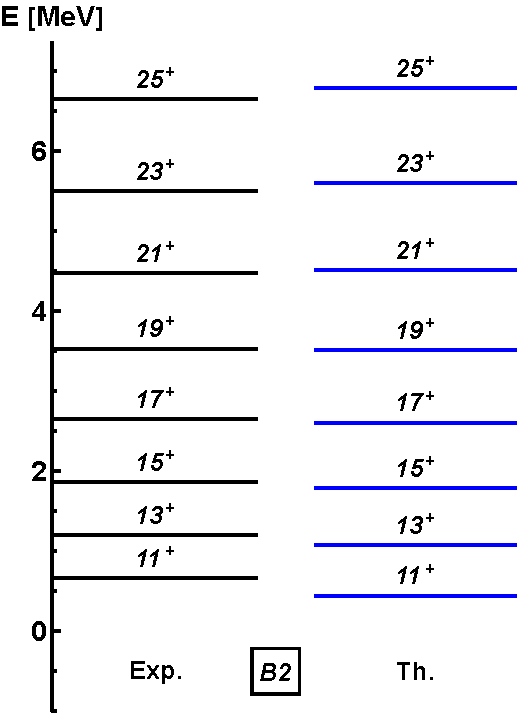
\includegraphics[width=0.46\textwidth]{Chapters/Figures/ba130-band2.pdf}
    \caption{Comparison between the experimental and theoretical excitation energies (Eq. \ref{excitation-energy-general-formula}) for the two wobbling bands of $^{130}$Ba (B1 and B2). Experimental data are taken from Ref. \cite{petrache2019diversity}. The theoretical data was obtained by fitting Eq. \ref{eq-wobbling-energy-evenA} as described in text, with the parameters defined in Table \ref{table-params-ba130}. Note that the band-head $I^\pi=10^+$ state from B1 is missing from the spectrum, since it was subtracted from each level.}
    \label{plot-ba130-excitation-energies}
\end{figure}

Besides the excited spectrum obtained in Fig. \ref{plot-ba130-excitation-energies}, other quantities such as the rotational frequency (Eq. \ref{rotational-frequency-canonical}) for the two bands in $^{130}$Ba are compared with experimental values in Fig. \ref{wobbling-energies-130ba-expVSth}, and the obtained results agree with the measured data quite well. Note that both frequencies are increasing functions of angular momentum, although for B1, at spin $I\geq 24\hbar$, there seems to be a less of an increase, which is not fully reproduced by the fitted values. Moreover, having the excitation energies for the two bands, one can evaluate the theoretical wobbling energies as defined in Eq. \ref{eq-wobbling-energy-definition-oddA} and compare them with the experimental values. The two quantities are graphically represented in Fig. \ref{wobbling-energies-130ba-expVSth}. Remarking the fact that there is an opposite behavior for the two curves, namely the experimental wobbling energies decrease with angular momentum, while the theoretical ones are constantly increasing. Unfortunately, it turns out that by using the Hamiltonian for a \emph{simple wobbler} is not enough to completely describe the collective motion in this isotope.

\begin{figure}
    \centering
    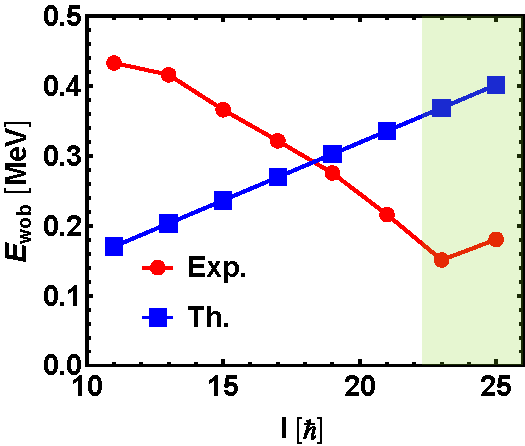
\includegraphics[scale=0.8]{Chapters/Figures/ba130-wobbling-energies-edited.pdf}
    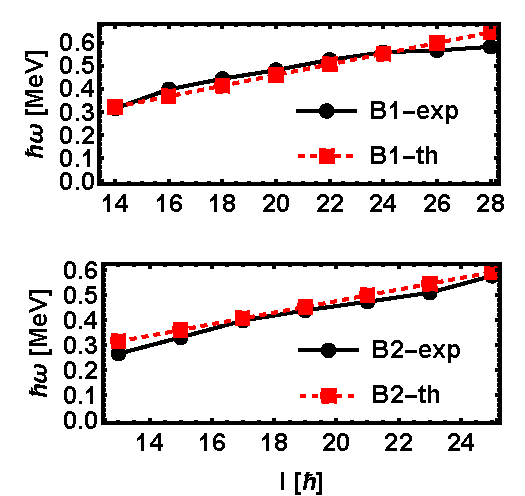
\includegraphics[scale=0.75]{Chapters/Figures/ba130-rotational-frequencies.pdf}
    \caption{\textbf{Left:} The wobbling energies for $^{130}$Ba calculated with Eq. \ref{eq-wobbling-energy-definition-oddA} (see text for explanation on the green region). For the first state of B2, the energy was determined as $E_\text{wob}(11^+)=E_\text{B2}(11^+)-\frac{1}{2}E_\text{B1}(12^+)$ since the band-head state of B1 is zero (as per the definition of excitation energy given in Eq. \ref{excitation-energy-general-formula}). \textbf{Right:} The rotational frequencies for the two wobbling bands of $^{130}$Ba, calculated using Eq. \ref{rotational-frequency-canonical}.}
    \label{wobbling-energies-130ba-expVSth}
\end{figure}

\subsubsection{Transition Probabilities}

Another step regarding the calculations for $^{130}$Ba consists of the electromagnetic transition probabilities. For this investigation some prior quantities are required. Firstly, the reduced transition probabilities $B(E2)$ (both the interband and the intraband) depend on the components $Q_{20}$ and $Q_{22}$ of the quadrupole moment. These two can be evaluated numerically using the expressions from Eq. \ref{quadrupole-components-q20-q22}, while the intrinsic quadrupole moment is furthermore evaluated using Eq. \ref{quadrupole-moment-Q0}. From the microscopic calculations performed by Chen et al. in Ref. \cite{chen2019transverse}, they determined that this isotope has a stable triaxial minimum located at $(\beta_2,\gamma)=(0.24,21.5^\circ)$. Within the following computations, this set of deformation parameters will be used. Taking the value of $\beta_2=0.24$, the intrinsic quadrupole moment $Q_0$ is readily obtained from Eq. \ref{quadrupole-moment-Q0}. The transition probabilities from Eqs. \ref{intraband-probability-simple-wobbler}, \ref{interband-probability-simple-wobbler-1}, and \ref{interband-probability-simple-wobbler-2} also depend on the two factors $w_{1,2}$ defined in Eq. \ref{eqs-w1-w2-terms-wobbling}, which are functions of the three moments of inertia. Thus, the quality of the fitting procedure will also reflect the calculus for the transition probabilities through $\mathcal{P}_\text{fit}$. The numerical values for $Q_0$, $w_{1,2}$, and $Q_{20,22}$ are presented in Table \ref{transition-parameters-ba130}. Having the deformation parameters, the $w_{1,2}$ terms, and the quadrupole components, one can evaluate the reduced transition probabilities. 

\begin{table}
    \centering
    \begin{tabular}{|c|c|c|}
    % \begin{tabular}{|p{0.15\linewidth}|p{0.25\linewidth}|p{0.5\linewidth}|}
    \hline
    Parameters & Calculated values & Observations                                               \\ \hline
    $\beta_2$  & 0.24              & Taken from Ref. \cite{chen2019transverse}                 \\ \hline
    $\gamma$   & $21.4^\circ$      & Taken from Ref. \cite{chen2019transverse}                 \\ \hline
    $w_1$      & 1.008             & Evaluated with $\mathcal{P}_\text{fit}$                    \\ \hline
    $w_2$      & 0.132             & Evaluated with $\mathcal{P}_\text{fit}$                    \\ \hline
    $Q_0$      & 390.376 $eb\cdot10^{-2}$      & As per Eq. \ref{quadrupole-moment-Q0}                                                           \\ \hline
    $Q_{20}$   & 363.213 $eb\cdot10^{-2}$          & As per Eq. \ref{quadrupole-components-q20-q22}                                                            \\ \hline
    $Q_{22}$   & 101.168 $eb\cdot10^{-2}$           & As per Eq. \ref{quadrupole-components-q20-q22}                                                            \\ \hline
    $B(E2)_\text{in}$ &        0.0509 $(eb)^2$          & Eq. \ref{intraband-probability-simple-wobbler}              \\ \hline
    \end{tabular}%
    \caption{The numerical values for the quantities which are required to determine the quadrupole transition probabilities $B(E2)$ defined in Eqs. \ref{intraband-probability-simple-wobbler} - \ref{interband-probability-simple-wobbler-2}. The parameter set $\mathcal{P}_\text{fit}$ was obtained through the fitting procedure and the values are shown in Table \ref{table-params-ba130}. The intraband transition probabilities $B(E2)$ are evaluated for states $(n,I)\to(,,I-2)$.}
    \label{transition-parameters-ba130}
\end{table}

The graphical representation from Fig. \ref{BE2out-transitions-130ba} shows the interband transition probabilities $B(E2)_\text{out}$ for states $(n_w=1,I)\to(n_w=0,I-1)$. These values are determined with the parameters defined in Table \ref{transition-parameters-ba130}. A constant decrease with spin can be observed, and an overall agreement with theoretical calculations from Ref. \cite{chen2019transverse} is observed (see inset $a$ from Fig. 4 in \cite{chen2019transverse}).

\begin{figure}
    \centering
    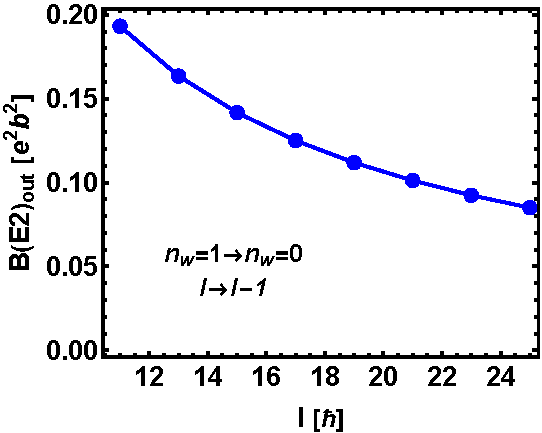
\includegraphics[scale=0.75]{Chapters/Figures/BE2-out-130Ba.pdf}
    \caption{The interband quadrupole transition probabilities (Eq. \ref{interband-probability-simple-wobbler-1}) from the first excited wobbling band (B2) to the yrast band (B1) for $^{130}$Ba.}
    \label{BE2out-transitions-130ba}
\end{figure}

Considering the interband transitions $B(E2)_\text{out}$ calculated above and the constant value for $B(E2)_\text{in}$ (typical for the HA), the ratios $B(E2)_\text{out}/B(E2)_\text{in}$ can also be evaluated. These values are good indicators if a nucleus has a strong deformation and for collective behavior (such as the wobbling motion), they typically lie within $0.2\sim 0.5$. In Table \ref{BE2-out-in-ratio-130Ba}, the obtained ratios are compared with the experimental ones, where a decent agreement can be seen, and also a decreasing trend with spin can be observed.

\begin{table}
    \centering
    \begin{tabular}{|c|cc|}
    \hline
    \multirow{2}{*}{$I$} & \multicolumn{2}{c|}{$\frac{B(E2)_\text{out}}{B(E2)_\text{in}}$} \\ \cline{2-3} 
                         & \multicolumn{1}{c|}{Experimental}          & Calculated         \\ \hline
    11                   & \multicolumn{1}{c|}{}                      & 0.37           \\ \hline
    13                   & \multicolumn{1}{c|}{0.32}                  & 0.32           \\ \hline
    15                   & \multicolumn{1}{c|}{0.36}                  & 0.27           \\ \hline
    17                   & \multicolumn{1}{c|}{0.22}                  & 0.24           \\ \hline
    19                   & \multicolumn{1}{c|}{0.22}                  & 0.21           \\ \hline
    21                   & \multicolumn{1}{c|}{0.41}                  & 0.19           \\ \hline
    23                   & \multicolumn{1}{c|}{}                      & 0.18           \\ \hline
    25                   & \multicolumn{1}{c|}{}                      & 0.16           \\ \hline
    \end{tabular}%
    \caption{The ratios $\frac{B(E2)_\text{out}}{B(E2)_\text{in}}$ for $^{130}$Ba. The interband transitions signify the change from a state $I$ in B2 to a state $I-1$ in B1. The experimental data (where available) were taken from Ref. \cite{petrache2019diversity,chen2019transverse}.}
    \label{BE2-out-in-ratio-130Ba}
\end{table}

\subsubsection{General Discussion}

Even though the spectrum of this even-even nucleus has been quantitatively reproduced quite well and the values for the tree obtained MOI indicate a triaxial nucleus with main rotation around the third axis, it should not be considered a `realistic' tool in describing this isotope. This is because in another work, Chen et al. \cite{chen2019transverse} (followed quickly also by \cite{wang2020two}) found through microscopic calculations that the wobbling motion does not occur as per a pure triaxial rotator, but it emerges from the coupling of two quasi-particles $\pi(h_{11/2})^2$ with a triaxial core. In fact, their work shows that $^{130}$Ba is the first nucleus in which a configuration with two quasi-particles generates stable triaxial deformation through wobbling motion. Consequently, the numerical implementation performed here only shows that HA can be a suitable tool to show that $^{130}$Ba does behave as a wobbler, but this pure triaxial rotator model \emph{hides} contributions coming from single-particle configuration within the final Hamiltonian. This translates to the fact that Eq. \ref{eq-wobbling-energy-evenA} contains the effect of the two $h_{11/2}$ protons hidden within $\hbar\omega_w$. In fact, looking back at $E_\text{wob}$ from Fig. \ref{wobbling-energies-130ba-expVSth}, the discrepancy of the two lines is a clear indicator that some other terms should be taken into account. The experimental wobbling energy from Fig. \ref{wobbling-energies-130ba-expVSth} does show an increasing trend for large spins ($I\geq 23\hbar$) which is also matched by the theoretical model (the green region marked inside the plot), indicating some sort of \emph{transition} with respect to the motion of the nucleus. The transition between decreasing/increasing behavior will be discussed on the next section, dedicated to the odd-mass nuclei.

Also, it is worth mentioning that a quenching factor was necessary in the expression of $B(E2)_\text{in,out}$ in order to compensate for the magnitude of $w_{1,2}$. Nevertheless, this simple and straightforward formalism used to describe the wobbling bands in the even-even $^{130}$Ba nucleus proves to be a decent tool. The calculations presented here have been done independently by the current team, and the obtained results are unique to this research. They will be considered towards a separate forthcoming publication.

Concluding this section on wobbling motion of even-even nuclei, a final sketch is depicted in Fig. \ref{simple-wobbler-geometrical-schematic}, where the main axes of the triaxial ellipsoid are represented and denoted with $m$, $s$, and $l$-axis (medium, short and long, respectively). The precession motion of the total angular momentum (the a.m. of the core itself) will be around the $m$-axis, having the largest moment of inertia.

\begin{figure}
    \centering
    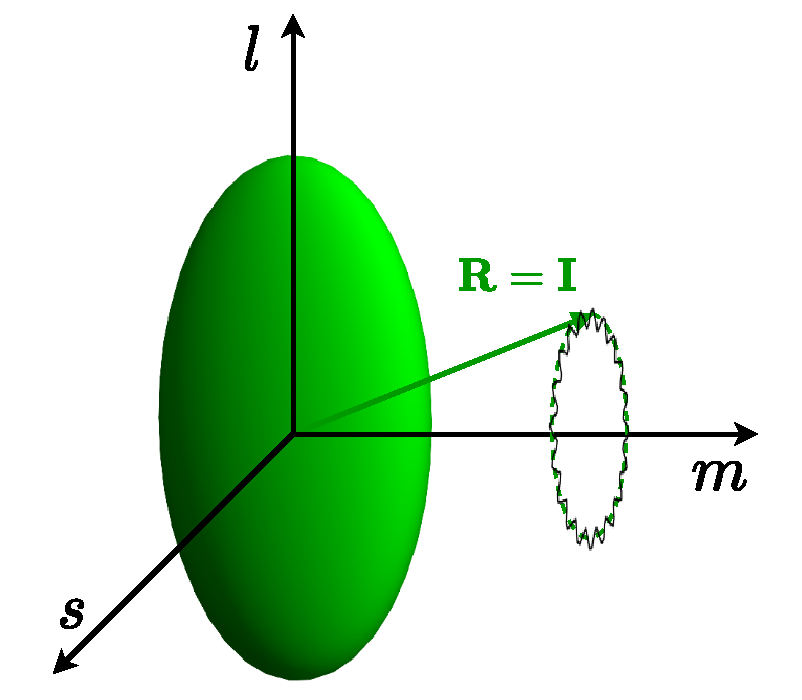
\includegraphics[scale=0.6]{Chapters/Figures/simple_wobbler-schematic.pdf}
    \caption{A schematic representation with a \emph{simple wobbler}, with the total angular momentum doing a precessional motion about the axis with the largest MOI. In this particular sketch, the axis with the largest MOI is denoted with $m$ for intermediate/medium. The long and short axes are represented by $l$ and $s$, respectively. The small-amplitude oscillations of $\mathbf{R}_\mathscr{C}$ are depicted with the (black) encircled sine wave. Notation of the angular momentum is consistent with Table \ref{notation-table-wobbling}. This figure was adapted from Ref. \cite{poenaru2021extensive1} and inspired from Ref. \cite{sensharma2020longitudinal}.}
    \label{simple-wobbler-geometrical-schematic}
\end{figure}

\section{Wobbling Motion in Odd-Mass Nuclei}

The previous discussion regarding the \emph{simple wobbler} was specific to nuclei with even number of nucleons. However, wobbling motion does also occur in odd-mass isotopes. In fact, it turns out that across the chart of nuclides, most of the wobblers are odd-$A$. The reason for this has to do with the triaxial nature of a nucleus. In simple terms, it is `easier' for a (non-axial) deformed system to achieve stability if there is a valence nucleon in a high-$j$ shell which couples to a triaxial core and then drives the entire system to large deformation (remember that different nucleon orbitals will favor specific $\gamma$ values for reaching stable minima).

As an example, for nuclei in the region $N\approx 94$, stable triaxial shapes with large deformations emerge (e.g., $\beta_2\approx0.4$.). These are built on the configuration in which an odd nucleon (i.e., the $i_{13/2}$ proton) couples to a triaxial even-even core. This highly aligned proton will play a crucial role in generating the wobbling excitations for these nuclei by driving the nuclear shape towards large deformations and stabilizing the TSD shapes. Based on this, the description for wobbling motion in an odd-mass system will require the usage of a typical Particle-Rotor-Model that was previously discussed. More precisely, since the core can couple with a particle or hole, and since the deformed system is triaxial, then a particle + triaxial rotor model is needed \cite{frauendorf2014transverse}. The model Hamiltonian can be expressed as:
\begin{align}
    \hat{H}_\text{QTR}=H_\text{coupl.}+\sum_{k=1}^{3}A_k(\hat{I}_k-\hat{j}_k)^2\ ,
    \label{oddA-QTR-general-hamiltonian}
\end{align}
where the odd quasi-particle's a.m. is denoted by $\hat{j}$ and the total a.m. is denoted by $\hat{I}_k$. $H_\text{coupl.}$ defines the coupling of the odd nucleon with the triaxial core. This model is known as \emph{Quasi-Particle Triaxial Rotor} (QTR) and it has been developed by Frauendorf et al. in Ref. \cite{frauendorf2014transverse} (the term quasi-particle adopted here signifies the fact that both a particle or a hole can similarity couple to the core). The Hamiltonian given in Eq. \ref{oddA-QTR-general-hamiltonian} (hereafter the subscript `QTR' from Eq. \ref{oddA-QTR-general-hamiltonian} will be dismissed) can be treated in the so-called \emph{Frozen Alignment} (FA) approximation \cite{frauendorf2014transverse}. The idea behind FA is that the a.m. for the quasi-particle is fixed (i.e., rigidly aligned) along one of the principal axes of $\mathscr{C}$. Frauendorf obtained a remarking property while describing the QTR Hamiltonian within FA approximations. Indeed, two possible wobbling modes can exist: the \emph{longitudinal wobbling} and \emph{transverse wobbling}. These two scenarios arise from the alignment done by the odd quasi-particle with the axis with the largest MOI of the triaxial core. The  quasi-particle + core system is regarded as a valence nucleon moving in a quadrupole deformed mean-field generated by the core, so the coupling term $H_\text{coupl.}$ can be considered a single-particle term as the one presented in Eqs. \ref{quadrupole-deformed-potential-beta}-\ref{single-particle-nilsson-defored-potential} or Eq. \ref{single-particle-energies-hpn}.

In order to avoid repeating certain words, some notations will be adopted throughout the following sections and chapters. Namely, the concept of quasi-particle will be denoted with $\mathcal{Q}$. Additionally, a quasi-particle with \emph{hole} character will be referred to as $\mathcal{Q}_h$ while a quasi-particle with \emph{particle} character will be labelled as $\mathcal{Q}_p$. Finally, the core will be denoted with $\mathscr{C}$. These notations can be seen in Table \ref{notation-table-wobbling}.
\begin{table}
    \centering
    \resizebox{0.8\textwidth}{!}{%
    \begin{tabular}{|c|c|c|}
    \hline
    Object                                                       & Notation                    & Angular momentum             \\ \hline
    quasi-particle                                                 & $\mathcal{Q}$               & $\mathbf{j}_{\mathcal{Q}}$   \\ \hline
    q-p with \emph{particle} character & $\mathcal{Q}_p$             & $\mathbf{j}_{\mathcal{Q}_p}$ \\ \hline
    q-p with \emph{hole} character     & $\mathcal{Q}_h$             & $\mathbf{j}_{\mathcal{Q}_h}$ \\ \hline
    triaxial even-even core                                        & $\mathscr{C}$               & $\mathbf{R}_\mathscr{C}$    \\ \hline
    total system                        & $\mathcal{Q}+\mathscr{C}$ & $\mathbf{I}$                             \\ \hline
    \end{tabular}%
    }
    \caption{The notations adopted for describing wobbling motion in odd-$A$ nuclei by means of particles and angular momenta. These symbols will be used throughout the rest of the work.}
    \label{notation-table-wobbling}
\end{table}

The stability of the triaxial nuclear shapes consists of existence of minima within the energy function (see discussion on PES given in Section \ref{potential-energy-surfaces-section}). In order to minimize the system's energy, a $\mathcal{Q}_p$ ($\mathcal{Q}_h$) will tend to create a specific coupling with $\mathscr{C}$, such that their density distribution overlap become maximal (minimal). A maximal (minimal) overlap for $\mathcal{Q}_p+\mathscr{C}$ ($\mathcal{Q}_h+\mathscr{C}$) will minimize the attractive (repulsive) short-range interaction between the two. In terms of the coupling, one can have \cite{frauendorf2014transverse}:
\begin{itemize}
    \item the angular momentum for a high-$j$ $\mathcal{Q}_p$ (i.e., $\mathbf{j}_{\mathcal{Q}_p}$) will align itself with the short ($s$-axis) of $\mathscr{C}$ 
    \item the angular momentum for a high-$j$ $\mathcal{Q}_h$ (i.e., $\mathbf{j}_{\mathcal{Q}_h}$) will make an alignment with the long ($l$-axis) of $\mathscr{C}$
    \item the angular momentum for any $\mathcal{Q}$ (i.e., $\mathbf{j}_{\mathcal{Q}}$) from a half-filled high-$j$ shell will align itself with the intermediate ($m$-axis) of $\mathscr{C}$
\end{itemize}
Going back to the discussion on longitudinal and transverse wobbling modes, it is the $\mathcal{Q}+\mathscr{C}$ coupling that dictates what wobbling mode will arise. More precisely, if the a.m. for $\mathcal{Q}$ aligns itself \emph{along} the $m$-axis, then the motion is considered \emph{longitudinal wobbling} (LW). On the other hand, if the a.m. for $\mathcal{Q}$ aligns itself \emph{perpendicular} to the $m$-axis, then the motion is considered as \emph{transverse wobbling} (TW). One can encounter two different situations that could lead to transverse wobbling. If a $\mathcal{Q}_p$ comes from the bottom of a deformed $j$-shell, it will align its a.m. with the $s$-axis (i.e., $s\perp m$). Moreover, if a $\mathcal{Q}_h$ comes from the top of a deformed $j$-shell, it will tend to align its a.m. with the $l$-axis (i.e., $l\perp m$), which is consistent with the discussion made in Section \ref{chiral-section}. These three scenarios are summarized in three \emph{workflow diagrams} that aim to depict the wobbling motion (stable triaxial structures), starting from the quasi-particle position within a $j$-shell and ending with the emerging wobbling behavior. For the TW case, one can see the sketches from Figs. \ref{advanced-quasiparticle-coupling-1}-\ref{advanced-quasiparticle-coupling-2}, while the same analogy is shown in Fig. \ref{advanced-quasiparticle-coupling-3} for LW.
\begin{figure}
    \centering
    \begin{tikzpicture}[every text node part/.style={align=center}]
        % draw a background box for the density overlap and the two gaussian curves
        \node[rectangle, very thick,dashed,draw=black,fill=none] (huge-container-box) [minimum height=5cm,minimum width=12cm,xshift=0.7cm,yshift=-0.3cm] at (2,2.5) {};
        \begin{scope}[xshift=1cm]
            % add coupling schematic
            \draw[-latex] [thick, color=black,dashed] (1.5,6) -- (6,6) node [yshift=-0.3cm] {$m$-axis};
            \draw[-latex] [ultra thick, color=black,dashed] (1.5,6) -- (6,6) node [yshift=+0.4cm,xshift=0.3cm] {$\mathcal{I}_m>(\mathcal{I}_{l},\mathcal{I}_{s})$};
            \draw[-latex] [thick, color=black,dashed] (1.5,6) -- (1.5,9) node [pos=1,above] {$s$-axis};
            \draw[-latex] [ultra thick, color=black!60!green] (1.5,6) -- (4,6.6) node [yshift=0.3cm,xshift=-0.5cm] {$\mathbf{R}_{\mathscr{C}}$};
            \draw[-latex] [ultra thick, color=magenta] (1.5,6) -- (1.5,8) node [xshift=-0.5cm] (my-arrow) {$\mathbf{j}_{\mathcal{Q}_p}$};
            % \draw[-latex] [ultra thick, color=magenta] (1.5,6) -- (1.5,8) node [pos=1,above,xshift=-1cm] (my-arrow) {$\mathbf{j}_{\mathcal{Q}_p}$};
            \node[rectangle, draw=black, fill=none,anchor=south west] at (1.5,6) {};
            \node[rectangle, draw=black, fill=green!10,anchor=south west, minimum width=4cm] at (3,7.5) (coupling-box) {$(\mathcal{Q}_p+\mathscr{C})$\\ Coupling};
        \end{scope}
        
        \node[rectangle, draw=black, thick, fill=green!10, inner sep=0.2cm,minimum width=8 cm] at (2,-1.8) (first-box) {\textbf{Minimized} short-range interaction \\ \\ $\mathcal{Q}_p+\mathscr{C}$ = \emph{attractive}};
        \node[rectangle] (pes-image-box) [right=of first-box,xshift=-0.7cm] {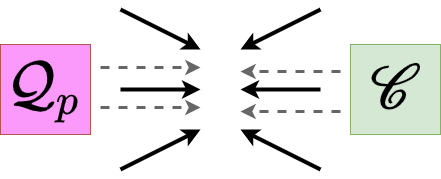
\includegraphics[scale=0.2]{Chapters/Figures/attractive_interaction.png}};
        
        \node[rectangle, draw=black, thick, fill=green!10, inner sep=0.2cm,minimum width=8 cm] (second-box) [below=of first-box] {\textbf{Minimal} energy (PES)};
        \node[rectangle] (pes-image-box) [right=of second-box,xshift=-0.7cm,yshift=0.4cm] {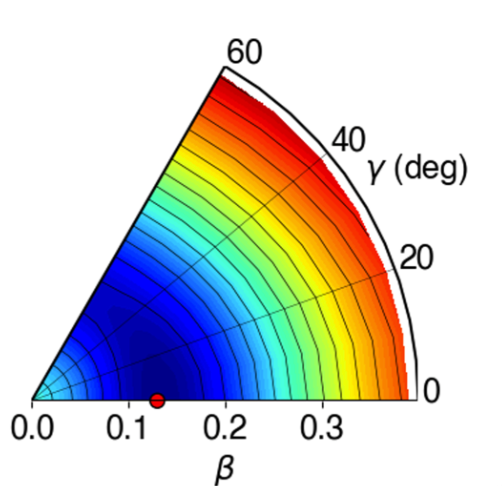
\includegraphics[scale=0.12]{Chapters/Figures/PES_small_update.png}};
        
        \node[rectangle, draw=black, thick, fill=green!10, inner sep=0.2cm,minimum width=8 cm] (third-box) [below=of second-box] {\textbf{Stable triaxial shape} \\ $\downarrow$ \\ \textbf{Transverse Wobbling Motion}: \\ $\mathbf{j}_{\mathcal{Q}_p}\perp \mathbf{m}_\text{axis}$};
        \node[rectangle] (precession-cone-box) [right=of third-box,xshift=-1cm] {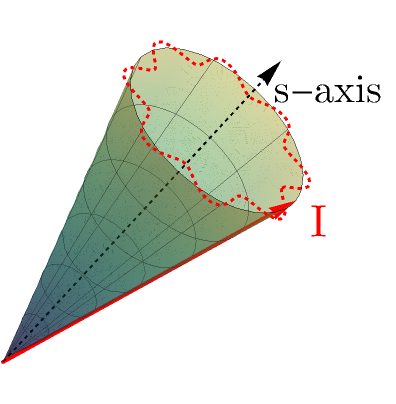
\includegraphics[scale=0.3]{Chapters/Figures/precessional_cone.png}};
        
        \node[rectangle, draw=black,xshift=6cm,yshift=2cm,fill=green!10, minimum width=4cm] (maximal-box) {\textbf{Maximal overlap} \\ between \\ {\color{magenta}$\mathcal{D}\left(\mathcal{Q}_p\right)$} and {\color{black!60!green}$\mathcal{D}\left(\mathscr{C}\right)$}};


        % \draw[-latex] [very thick,black] (inside-node.east) -- ($(inside-node.east)+(2.2,0)$) |- node [xshift=-1.9cm,yshift=2.7cm] (maximal-box) {\textbf{Maximal overlap} \\ between \\ {\color{magenta}$\mathcal{D}\left(\mathcal{Q}_p\right)$} and {\color{black!60!green}$\mathcal{D}\left(\mathscr{C}\right)$}} (first-box.east);
        % \draw[-latex] [very thick,black] (first-box) -- node[circle,draw=black,xshift=1cm] {a} (second-box);
        \draw[-latex] [very thick,black] (first-box) -- node[circle,draw=black,xshift=1cm,fill=yellow!30] {$4$} (second-box);
        \draw[-latex] [very thick,black] (second-box) -- node[circle,draw=black,xshift=1cm,fill=yellow!30] {$5$} (third-box);
        % \draw[-latex] [very thick, color=black] (1.5,5.5) -| (maximal-box.east);
        
        % draw arrow for coupling and maximal overlap
        \draw[-latex] [very thick, color=black] (coupling-box.east) -- ($(coupling-box.east)+(1,0)$) |- node[circle,draw=black,xshift=-0.4cm,yshift=-0.6cm,fill=yellow!30] {$2$} (maximal-box.east);

        \begin{axis}[scale=0.6,xshift=-2cm,every axis plot post/.append style={
            mark=none,domain=-2:3,samples=50,smooth}, % All plots: from -2:2, 50 samples, smooth, no marks
            axis x line*=bottom, % no box around the plot, only x and y axis
            axis y line*=left, % the * suppresses the arrow tips
            axis line style={draw=none},
            xtick=\empty, ytick=\empty,
            enlargelimits=false, 
            clip=false, 
            axis on top,
            grid = major,
            legend style={at={(1,1)},anchor=north,legend cell align=left}
            ]
            % extend the axes a bit to the right and top
            
            \addplot [name path=particle-density, color=magenta,ultra thick] {\gauss{0}{0.5}};
            \addplot [name path=core-density, color=black!60!green,ultra thick] {\gauss{0.4}{0.7}};
            \legend{$\mathcal{D}\left(\mathcal{Q}_p\right)$,$\mathcal{D}\left(\mathscr{C}\right)$}
            \path[name path=axis] (axis cs:1,0) -- (axis cs:2,0);
            
            % path for fixing boundaries which will be used to fill common region between gaussian curves
            \path[name path=lower,intersection segments={of=particle-density and core-density, sequence={L1 -- R2 -- L3}}];
            
            \node[rectangle, draw=none, thick, fill=none] at (axis cs: 0.8,0.9) (inside-node) {Density distributions for $\mathcal{Q}_p$ and $\mathscr{C}$};
            
            \addplot[color=gray!30] fill between[of= lower and axis];
        \end{axis}

        \begin{scope}[yshift=6cm,xshift=-4cm]
            % draw Fermi orbital for a j-particle
            \node[rectangle, very thick,draw=black,fill=yellow!50] (jshell-box) [minimum height=3cm,minimum width=2cm] at (2.5,1.5) {};
            \foreach \x [count=\xi] in {0.1,0.2,0.3,0.4,0.5,0.6} { 
                \draw (2,\xi em) -- (3,\xi em) ;
            }
            \node at (1.8,0.4) {$\mathcal{Q}_p$};
            \node[circle,draw=none,fill=magenta] at (2.5,0.4) {};
            \node[] at (2.5,-0.5) {$j$-shell};
        \end{scope}

        %draw arrow from jshell to coupling box
        \draw[-latex,very thick] (jshell-box.north) -- ($(jshell-box.north)+(0,1cm)$) node[circle,draw=black,yshift=-0.6cm,xshift=8.1cm,fill=yellow!30] {$1$} -| (coupling-box);

        % connect maximal overlap with minimal interaction
        \draw[-latex,very thick] (maximal-box.south) -- ($(maximal-box.south)-(0,0.4cm)$) -| node[draw=black,circle,yshift=-0.5cm,xshift=0.6cm,fill=yellow!30] {$3$} ([xshift=1cm]first-box.north);
    \end{tikzpicture}
    \caption{The workflow of a quasi-particle with particle character $\mathcal{Q}_p$ in its coupling with a triaxial rotor $\mathscr{C}$. Each of the five `steps' represents a characteristic involved in the wobbling motion, as described in text. Namely, for $\mathcal{Q}_p$ coming from the bottom of a $j$-shell and coupling with the $s$-axis of the even-even core $\mathscr{C}$ \textbf{(1)} will maximize the density overlap \textbf{(2)}, which will minimize their interaction \textbf{(3)}, minimizing the total energy \textbf{(4)}, and finally stabilizing the triaxial structure \textbf{(5)} to a TW. The long $l$-axis has been ignored within the drawings. In the bottom-most picture, the precessional cone of the total a.m. is shown, oscillating along the $s$-axis.}
    \label{advanced-quasiparticle-coupling-1}
\end{figure}
\begin{figure}
\centering
\begin{tikzpicture}[every text node part/.style={align=center}]
    % draw a background box for the density overlap and the two gaussian curves
    \node[rectangle, very thick,dashed,draw=black,fill=none] (huge-container-box) [minimum height=5cm,minimum width=12cm,xshift=0.7cm,yshift=-0.3cm] at (2,2.5) {};
    \begin{scope}[xshift=1cm]
        % add coupling schematic
        \draw[-latex] [thick, color=black,dashed] (1.5,6) -- (6,6) node [yshift=-0.3cm] {$m$-axis};
        \draw[-latex] [ultra thick, color=black,dashed] (1.5,6) -- (6,6) node [yshift=+0.4cm,xshift=0.3cm] {$\mathcal{I}_m>(\mathcal{I}_{l},\mathcal{I}_{s})$};
        \draw[-latex] [thick, color=black,dashed] (1.5,6) -- (1.5,9) node [pos=1,above] {$l$-axis};
        \draw[-latex] [ultra thick, color=black!60!green] (1.5,6) -- (4,6.6) node [yshift=0.3cm,xshift=-0.5cm] {$\mathbf{R}_{\mathscr{C}}$};
        \draw[-latex] [ultra thick, color=blue] (1.5,6) -- (1.5,8) node [xshift=-0.5cm] (my-arrow) {$\mathbf{j}_{\mathcal{Q}_h}$};
        % \draw[-latex] [ultra thick, color=magenta] (1.5,6) -- (1.5,8) node [pos=1,above,xshift=-1cm] (my-arrow) {$\mathbf{j}_{\mathcal{Q}_p}$};
        \node[rectangle, draw=black, fill=none,anchor=south west] at (1.5,6) {};
        \node[rectangle, draw=black, fill=red!10,anchor=south west, minimum width=4cm] at (3,7.5) (coupling-box) {$(\mathcal{Q}_h+\mathscr{C})$\\ Coupling};
    \end{scope}
    
    \node[rectangle, draw=black, thick, fill=red!10, inner sep=0.2cm,minimum width=8 cm] at (2,-1.8) (first-box) {\textbf{Minimized} short-range interaction \\ \\ $(\mathcal{Q}_h+\mathscr{C})$ = \emph{repulsive}};
    \node[rectangle] (pes-image-box) [right=of first-box,xshift=-0.7cm] {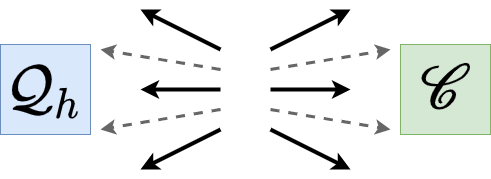
\includegraphics[scale=0.2]{Chapters/Figures/repulsive_interaction.png}};
    
    \node[rectangle, draw=black, thick, fill=red!10, inner sep=0.2cm,minimum width=8 cm] (second-box) [below=of first-box] {\textbf{Minimal} energy (PES)};
    \node[rectangle] (pes-image-box) [right=of second-box,xshift=-0.7cm,yshift=0.4cm] {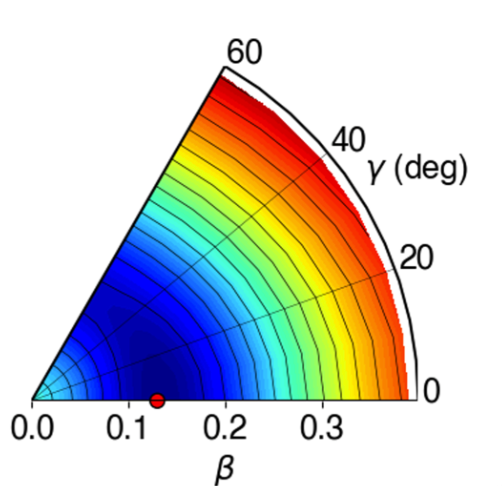
\includegraphics[scale=0.12]{Chapters/Figures/PES_small_update.png}};
    
    \node[rectangle, draw=black, thick, fill=red!10, inner sep=0.2cm,minimum width=8 cm] (third-box) [below=of second-box] {\textbf{Stable triaxial shape} \\ $\downarrow$ \\ \textbf{Transverse Wobbling Motion}: \\ $\mathbf{j}_{\mathcal{Q}_h}\perp \mathbf{m}_\text{axis}$};
    \node[rectangle] (precession-cone-box) [right=of third-box,xshift=-1cm] {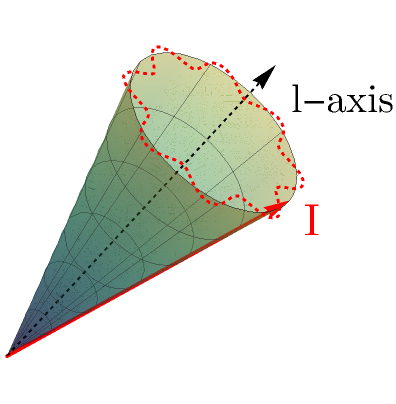
\includegraphics[scale=0.3]{Chapters/Figures/precessional_cone_2.png}};
    
    \node[rectangle, draw=black,xshift=6cm,yshift=2cm,fill=red!10, minimum width=4cm] (maximal-box) {\textbf{Minimal overlap} \\ between \\ {\color{blue}$\mathcal{D}\left(\mathcal{Q}_h\right)$} and {\color{black!60!green}$\mathcal{D}\left(\mathscr{C}\right)$}};


    % \draw[-latex] [very thick,black] (inside-node.east) -- ($(inside-node.east)+(2.2,0)$) |- node [xshift=-1.9cm,yshift=2.7cm] (maximal-box) {\textbf{Maximal overlap} \\ between \\ {\color{magenta}$\mathcal{D}\left(\mathcal{Q}_p\right)$} and {\color{black!60!green}$\mathcal{D}\left(\mathscr{C}\right)$}} (first-box.east);
    % \draw[-latex] [very thick,black] (first-box) -- node[circle,draw=black,xshift=1cm] {a} (second-box);
    \draw[-latex] [very thick,black] (first-box) -- node[circle,draw=black,xshift=1cm,fill=yellow!30] {$4$} (second-box);
    \draw[-latex] [very thick,black] (second-box) -- node[circle,draw=black,xshift=1cm,fill=yellow!30] {$5$} (third-box);
    % \draw[-latex] [very thick, color=black] (1.5,5.5) -| (maximal-box.east);
    
    % draw arrow for coupling and maximal overlap
    \draw[-latex] [very thick, color=black] (coupling-box.east) -- ($(coupling-box.east)+(1,0)$) |- node[circle,draw=black,xshift=-0.4cm,yshift=-0.6cm,fill=yellow!30] {$2$} (maximal-box.east);

    \begin{axis}[scale=0.6,xshift=-2cm,every axis plot post/.append style={
        mark=none,
        domain=0:10,
        samples=50,
        smooth}, % All plots: from -3:3, 50 samples, smooth, no marks
        axis x line*=bottom, % no box around the plot, only x and y axis
        axis y line*=left, % the * suppresses the arrow tips
        axis line style={draw=none},
        xtick=\empty, ytick=\empty,
        enlargelimits=false, 
        clip=false, 
        grid = major,
        legend style={at={(1,1)},anchor=north,legend cell align=left}
        ]
        % extend the axes a bit to the right and top
        
        % \addplot [name path=particle-density, color=blue,very thick] {\gauss{5}{0.4}};
        % \addplot [name path=core-density, color=black!60!green,very thick] {\gauss{5}{0.65}};
        
        % use filling implementation from this pose 
        % source: https://tex.stackexchange.com/a/305677/139074

        \addplot [name path=model,ultra thick, smooth, color=blue] {\gauss{3}{1}};
        \addplot [name path=obs,ultra thick, smooth, color=black!60!green] {\gauss{6.5}{1.2}};
        \legend{$\mathcal{D}\left(\mathcal{Q}_h\right)$,$\mathcal{D}\left(\mathscr{C}\right)$}
        
        \node[rectangle, draw=none, thick, fill=none] at (axis cs: 5.3,0.48) (inside-node) {Density distributions for $\mathcal{Q}_n$ and $\mathscr{C}$};

        \path[name path=lower,
        intersection segments={
        of=model and obs,
        sequence=A0 -- B1}];

        \path[name path=axis] (axis cs:0,0) -- (axis cs:16,0);

        \addplot[color=gray!30]
        fill between[
        of= model and axis]
        ;
        \addplot[color=white]
        fill between[
        of=model and obs,
        soft clip={domain=0:10}]
        ;

    \end{axis}

    \begin{scope}[yshift=6cm,xshift=-4cm]
        % draw Fermi orbital for a j-particle
        \node[rectangle, very thick,draw=black,fill=yellow!50] (jshell-box) [minimum height=3cm,minimum width=2cm] at (2.5,1.5) {};
        \foreach \x [count=\xi] in {0.1,0.2,0.3,0.4,0.5,0.6} { 
            \draw (2,\xi em) -- (3,\xi em) ;
        }
        \node at (1.8,2.5) {$\mathcal{Q}_h$};
        \node[circle,draw=none,fill=blue] at (2.5,2.5) {};
        \node[] at (2.5,-0.5) {$j$-shell};
    \end{scope}

    %draw arrow from jshell to coupling box
    \draw[-latex,very thick] (jshell-box.north) -- ($(jshell-box.north)+(0,1cm)$) node[circle,draw=black,yshift=-0.6cm,xshift=8.1cm,fill=yellow!30] {$1$} -| (coupling-box);

    % connect maximal overlap with minimal interaction
    \draw[-latex,very thick] (maximal-box.south) -- ($(maximal-box.south)-(0,0.4cm)$) -| node[draw=black,circle,yshift=-0.5cm,xshift=0.6cm,fill=yellow!30] {$3$} ([xshift=1cm]first-box.north);
\end{tikzpicture}
\caption{The workflow of a quasi-particle with hole character $\mathcal{Q}_h$ in its coupling with a triaxial rotor $\mathscr{C}$. Each of the five `steps' represents a characteristic involved in the wobbling motion, as described in text. Namely, for $\mathcal{Q}_h$ coming from the top of a $j$-shell and coupling with the $l$-axis of the even-even core $\mathscr{C}$ \textbf{(1)} will minimize the density overlap \textbf{(2)}, which will minimize their interaction \textbf{(3)}, minimizing the total energy \textbf{(4)}, and finally stabilizing the triaxial structure \textbf{(5)} to a TW. The short $s$-axis has been ignored within the drawings. In the bottom-most picture, the precessional cone of the total a.m. is shown, oscillating along the $l$-axis.}
\label{advanced-quasiparticle-coupling-2}
\end{figure}
\begin{figure}
    \centering
    \begin{tikzpicture}[every text node part/.style={align=center}]
        
        % draw a background box for the density overlap and the two gaussian curves
        \node[rectangle, very thick,dashed,draw=black,fill=none] (huge-container-box) [minimum height=5cm,minimum width=12cm,xshift=0.7cm,yshift=-0.3cm] at (2,2.5) {};
        
        \begin{scope}[xshift=1cm]
            % add coupling schematic
            \draw[-latex] [thick, color=black,dashed] (1.5,6) -- (5.5,6) node [yshift=-0.3cm] {$m$-axis};
            \draw[-latex] [ultra thick, color=black,dashed] (1.5,6) -- (6,6) node [yshift=+0.4cm,xshift=0.3cm] {$\mathcal{I}_m>(\mathcal{I}_{l},\mathcal{I}_{s})$};
            % \draw[-latex] [thick, color=black,dashed] (1.5,6) -- (1.5,9) node [pos=1,above] {$l$-axis};
            \draw[-latex] [ultra thick, color=black!60!green] (1.5,6) -- (4,6.6) node [yshift=0.3cm,xshift=-0.5cm] {$\mathbf{R}_{\mathscr{C}}$};
            \draw[-latex] [ultra thick, color=magenta] (1.5,6) -- (3,6) node [yshift=-0.4cm] (my-arrow) {$\mathbf{j}_{\mathcal{Q}_p}$};
            \node[rectangle, draw=black, fill=blue!10,anchor=south west, minimum width=4cm] at (3,7.5) (coupling-box) {$(\mathcal{Q}_p+\mathscr{C})$\\ Coupling};
        \end{scope}
        
        \node[rectangle, draw=black, thick, fill=blue!10, inner sep=0.2cm,minimum width=8 cm] at (2,-1.8) (first-box) {\textbf{Minimized} short-range interaction \\ \\ $(\mathcal{Q}_p+\mathscr{C})$ = \emph{attractive}};
        \node[rectangle] (pes-image-box) [right=of first-box,xshift=-0.7cm] {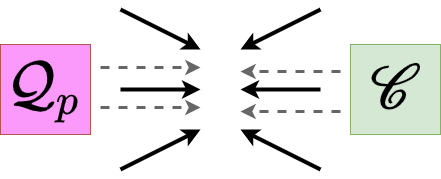
\includegraphics[scale=0.2]{Chapters/Figures/attractive_interaction.png}};
        
        \node[rectangle, draw=black, thick, fill=blue!10, inner sep=0.2cm,minimum width=8 cm] (second-box) [below=of first-box] {\textbf{Minimal} energy (PES)};
        \node[rectangle] (pes-image-box) [right=of second-box,xshift=-0.7cm,yshift=0.4cm] {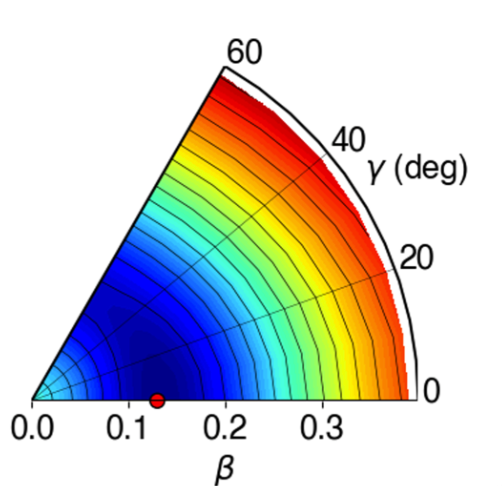
\includegraphics[scale=0.12]{Chapters/Figures/PES_small_update.png}};
        
        \node[rectangle, draw=black, thick, fill=blue!10, inner sep=0.2cm,minimum width=8 cm] (third-box) [below=of second-box] {\textbf{Stable triaxial shape} \\ $\downarrow$ \\ \textbf{Longitudinal Wobbling Motion}: \\ $\mathbf{j}_{\mathcal{Q}_p}\ ||\ \mathbf{m}_\text{axis}$};
        \node[rectangle] (precession-cone-box) [right=of third-box,xshift=-1cm] {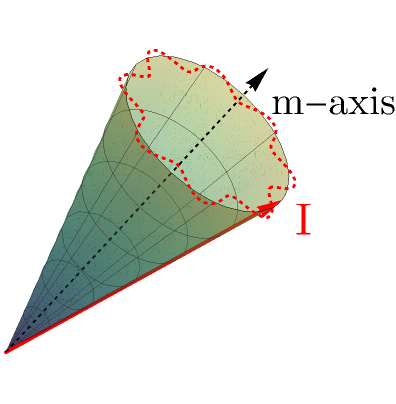
\includegraphics[scale=0.3]{Chapters/Figures/precessional_cone_3.png}};
        
        \node[rectangle, draw=black,xshift=6cm,yshift=2cm,fill=blue!10, minimum width=4cm] (maximal-box) {\textbf{Maximal overlap} \\ between \\ {\color{magenta}$\mathcal{D}\left(\mathcal{Q}_p\right)$} and {\color{black!60!green}$\mathcal{D}\left(\mathscr{C}\right)$}};


        % \draw[-latex] [very thick,black] (inside-node.east) -- ($(inside-node.east)+(2.2,0)$) |- node [xshift=-1.9cm,yshift=2.7cm] (maximal-box) {\textbf{Maximal overlap} \\ between \\ {\color{magenta}$\mathcal{D}\left(\mathcal{Q}_p\right)$} and {\color{black!60!green}$\mathcal{D}\left(\mathscr{C}\right)$}} (first-box.east);
        % \draw[-latex] [very thick,black] (first-box) -- node[circle,draw=black,xshift=1cm] {a} (second-box);
        \draw[-latex] [very thick,black] (first-box) -- node[circle,draw=black,xshift=1cm,fill=yellow!30] {$4$} (second-box);
        \draw[-latex] [very thick,black] (second-box) -- node[circle,draw=black,xshift=1cm,fill=yellow!30] {$5$} (third-box);
        % \draw[-latex] [very thick, color=black] (1.5,5.5) -| (maximal-box.east);
        
        % draw arrow for coupling and maximal overlap
        \draw[-latex] [very thick, color=black] (coupling-box.east) -- ($(coupling-box.east)+(1,0)$) |- node[circle,draw=black,xshift=-0.4cm,yshift=-0.6cm,fill=yellow!30] {$2$} (maximal-box.east);

        \begin{axis}[scale=0.6,xshift=-2cm,every axis plot post/.append style={
            mark=none,
            domain=0:10,
            samples=50,
            smooth}, % All plots: from -3:3, 50 samples, smooth, no marks
            axis x line*=bottom, % no box around the plot, only x and y axis
            axis y line*=left, % the * suppresses the arrow tips
            axis line style={draw=none},
            xtick=\empty, ytick=\empty,
            enlargelimits=false, 
            clip=false, 
            grid = major,
            legend style={at={(1,1)},anchor=north,legend cell align=left}
            ]
            % extend the axes a bit to the right and top
            
            % \addplot [name path=particle-density, color=blue,very thick] {\gauss{5}{0.4}};
            % \addplot [name path=core-density, color=black!60!green,very thick] {\gauss{5}{0.65}};
            
            % use filling implementation from this pose 
            % source: https://tex.stackexchange.com/a/305677/139074

            \addplot [name path=model,ultra thick, smooth, color=magenta] {\gauss{2.8}{1}};
            \addplot [name path=obs,ultra thick, smooth, color=black!60!green] {\gauss{3.5}{1.3}};
            \legend{$\mathcal{D}\left(\mathcal{Q}_p\right)$,$\mathcal{D}\left(\mathscr{C}\right)$}
            
            \node[rectangle, draw=none, thick, fill=none] at (axis cs: 5.3,0.48) (inside-node) {Density distributions for $\mathcal{Q}_p$ and $\mathscr{C}$};


            \path[name path=lower,
            intersection segments={
            of=model and obs,
            sequence=A0 -- B1}];

            \path[name path=axis] (axis cs:0,0) -- (axis cs:16,0);

            \addplot[color=gray!30]
            fill between[
            of= model and axis]
            ;
            \addplot[color=white]
            fill between[
            of=model and obs,
            soft clip={domain=0:10}]
            ;

        \end{axis}

        \begin{scope}[yshift=6cm,xshift=-4cm]
            % draw Fermi orbital for a j-particle
            \node[rectangle, very thick,draw=black,fill=yellow!50] (jshell-box) [minimum height=3cm,minimum width=2cm] at (2.5,1.5) {};
            \foreach \x [count=\xi] in {0.1,0.2,0.3,0.4,0.5,0.6} { 
                \draw (2,\xi em) -- (3,\xi em) ;
            }
            \node at (1.8,1.25) {$\mathcal{Q}_p$};
            \node[circle,draw=none,fill=magenta] at (2.5,1.25) {};
            \node[] at (2.5,-0.5) {$j$-shell};
        \end{scope}

        %draw arrow from jshell to coupling box
        \draw[-latex,very thick] (jshell-box.north) -- ($(jshell-box.north)+(0,1cm)$) node[circle,draw=black,yshift=-0.6cm,xshift=8.1cm,fill=yellow!30] {$1$} -| (coupling-box);

        % connect maximal overlap with minimal interaction
        \draw[-latex,very thick] (maximal-box.south) -- ($(maximal-box.south)-(0,0.4cm)$) -| node[draw=black,circle,yshift=-0.5cm,xshift=0.6cm,fill=yellow!30] {$3$} ([xshift=1cm]first-box.north);
    
    \end{tikzpicture}
    
    \caption{The workflow of a particle $\mathcal{Q}_p$ in its coupling with a triaxial rotor $\mathscr{C}$ within LW mode. Each of the five `steps' represents a characteristic involved in the wobbling motion, as described in text. Namely, for $\mathcal{Q}_p$ coming from the middle of a $j$-shell and coupling with the $m$-axis of the even-even core $\mathscr{C}$ \textbf{(1)} will maximize the density overlap \textbf{(2)}, which will minimize their interaction \textbf{(3)}, minimizing the total energy \textbf{(4)}, and finally stabilizing the triaxial structure \textbf{(5)}. In the bottom-most picture, the precessional cone of the total a.m. is shown, oscillating along the $m$-axis.}
    \label{advanced-quasiparticle-coupling-3}
\end{figure}

For increasing rotating motion, the Coriolis effect kicks in, trying to align the angular momentum of $\mathcal{Q}$ with the axis of rotation (i.e., the $m$-axis), creating thus a change from $(s)\to (m)$-axis for $\mathcal{Q}_p$ and a realignment $(l) \to (m)$-axis for $\mathcal{Q}_h$. The realignment will result in a transition from one wobbling regime to another, meaning that the system will undergo a phase transition. This kind of change can take place at some `critical' value for the nuclear spin $I$. In a recent work made by this team \cite{poenaru2021extensive1,poenaru2021extensive2} such a transition is discussed within a semi-classical approach. However, the FA approximation makes a constraint on the quasi-particle, meaning that its angular momentum is always aligned along one of the principal axes of the triaxial ellipsoid. Consequently, the Coriolis effect is left out when discussing TW or LW behavior and a change in regime caused by Coriolis effect will make the transverse/longitudinal wobbling motion to become unstable.

Returning to the QTR Hamiltonian from Eq. \ref{oddA-QTR-general-hamiltonian}, if one applies a small-amplitude limit for wobbling vibrations about the three-axis (i.e., a Harmonic Approximation such as the one used for the simple wobbler), and also the quasi-particle $\mathcal{Q}$ is fixed along the three-axis (making it \emph{frozen}), then the Hamiltonian will acquire the following form:
\begin{align}
    \hat{H}=A_3(\hat{I}_3-j)^2+A_1\hat{I}_1^2+A_2\hat{I}_2^2\ .
    \label{hamiltonian-qtr-FA}
\end{align}
By using such a constraint in the QTR Hamiltonian, the angular momentum for $\mathcal{Q}$ becomes just a number (i.e., $\mathbf{j}_{\mathcal{Q}}\to j$). Unless it is specifically mentioned, when $j$ appears in equations, it represents the angular momentum value of the fixed quasi-particle, and not the vector $\mathbf{j}_\mathcal{Q}$. Regarding the angular momentum components, these can be re-written as:
\begin{align}
    \hat{I}_3=\sqrt{\mathscr{I}^2-\hat{I}_1^2-\hat{I}_1^2}\approx\mathscr{I}-\frac{1}{2}\left(\frac{\hat{I}_1^2}{\mathscr{I}}+\frac{\hat{I}_2^2}{\mathscr{I}}\right)\ ,
\end{align}
where the `eigenvalue' of $\mathbf{I}$ is denoted as $\mathscr{I}=\sqrt{I(I+1)}$. Note that this is in fact a second-order expansion in terms of the square-root function. If the factor $A_3$ is also expressed in terms of $j$ and $\mathscr{I}$ (e.g., introducing a \emph{reduced} inertia parameter) via the relation:
\begin{align}
    \mathscr{A}_3=A_3\left(1-\frac{j}{\mathscr{I}}\right)\ ,
    \label{reduced-inertia-parameter-A3}
\end{align}
then the QTR Hamiltonian achieves the following form:
\begin{align}
    \hat{H}={\color{black}A_3(\mathscr{I}-j)^2}+{\color{black}(A_1-\mathscr{A}_3)\hat{I}_1^2+(A_2-\mathscr{A}_3)\hat{I}_2^2}\ .
    \label{HA-QTR-Hamiltonian}
\end{align}

The reduced inertia parameter $\mathscr{A}_3$ is graphically represented in Fig. \ref{reduced-inertia-A3-figs}, where the evolution w.r.t. spin is studied for different values of $A_3$ but fixed $j$ (left inset) and fixed $A_3$ but different $j$ (right inset). Keep in mind that the value of the spin $I$ defines the quantity $\mathscr{I}$ which enters in Eq. \ref{reduced-inertia-parameter-A3}.
\begin{figure}
    \centering
    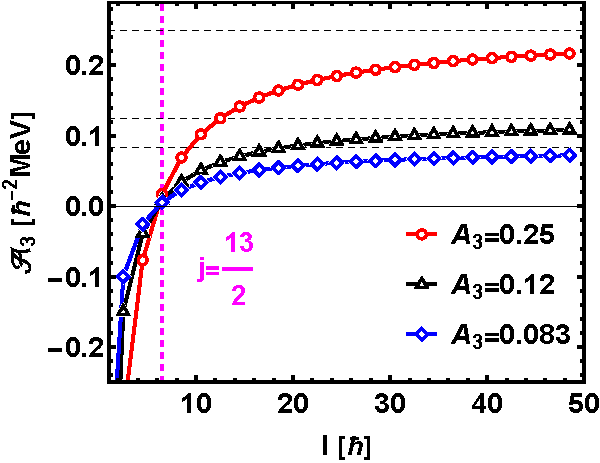
\includegraphics[width=0.49\textwidth]{Chapters/Figures/reducedInertia_fig1.pdf}
    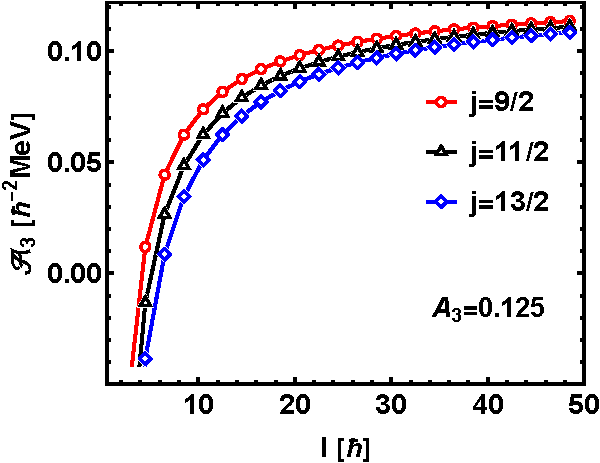
\includegraphics[width=0.49\textwidth]{Chapters/Figures/reducedInertia_fig2.pdf}
    \caption{The reduced inertia parameter defined in Eq. \ref{reduced-inertia-parameter-A3} as a function of spin. \textbf{Left:} The angular momentum of the quasi-particle is fixed (i.e., $j=13/2$) and different values for $A_3$ are attributed. The vertical grid-line corresponds to the value of $j$ at which $\mathscr{A}_3$ becomes positive. The horizontal dotted grid-lines correspond to the numerical values of $A_3$. \textbf{Right:} The value of $A_3$ is fixed and different a.m. values for $j$ are considered. Note that $I$ is used to define $\mathscr{I}$ which appears in the expression of $\mathscr{A}_3$.}
    \label{reduced-inertia-A3-figs}
\end{figure}

The Hamiltonian for an odd-$A$ triaxial nucleus has an expression which at a first glance looks quite similar to the simple wobbler (Eq. \ref{general-rotor-ham-evenA}), except that the coefficients of the first and second components $\hat{I}_{1,2}$ of the total a.m. contain a contribution coming from the quasi-particle itself (through the `reduced' inertia parameter $\mathscr{A}_3$ given in Eq. \ref{reduced-inertia-parameter-A3}). It is important to mention the fact that one can typically apply HA method for the QTR Hamiltonian only when $\hat{I}_1^2+\hat{I}_2^2<<I(I+1)$ \cite{bohr1998nuclear,frauendorf2014transverse}.

As it was the case for the simple wobbler (recall Eq. \ref{wobbling-frequency-even-A}), a wobbling frequency can be deduced from Eq. \ref{HA-QTR-Hamiltonian} by following a similar procedure. Thus, through an analogy with Eq. \ref{wobbling-frequency-even-A}, the QTR frequency is:
\begin{align}
    \hbar\omega_w=2\mathscr{I}\sqrt{\left(A_1-\mathscr{A}_3\right)\left(A_2-\mathscr{A}_3\right)}\ ,
    \label{wobbling-frequency-odd-A-inertiaParams}
\end{align}
or by expressing the factors $A_k$ in terms of the three moments of inertia:
\begin{align}
    \hbar\omega_w=\frac{j}{\mathcal{I}_3}\sqrt{\left[1+\frac{\mathscr{I}}{j}\left(\frac{\mathcal{I}_3}{\mathcal{I}_1}-1\right)\right]\left[1+\frac{\mathscr{I}}{j}\left(\frac{\mathcal{I}_3}{\mathcal{I}_2}-1\right)\right]}\ .
    \label{wobbling-frequency-odd-A-MOI}
\end{align}
The wobbling frequency for a longitudinal wobbler requires the condition:
\begin{align}
    \mathcal{I}_3>(\mathcal{I}_1,\mathcal{I}_1)\ \equiv\ A_3<(A_1,A_2)\ ,
\end{align}
meaning that the total system rotates around the $3$-axis (intermediate axis with largest MOI as $\mathcal{I}_3=\mathcal{I}_m$). For LW, both the $(\mathcal{I}_3/\mathcal{I}_1-1)$ and $(\mathcal{I}_3/\mathcal{I}_2-1)$ are positive, meaning that the wobbling frequency increases with $I$.
For the transverse wobbling, the MOI condition requires:
\begin{align}
    \mathcal{I}_3>\mathcal{I}_1\ \text{and}\ \mathcal{I}_3<\mathcal{I}_2\ ,
\end{align}
or, equivalently:
\begin{align}
    A_3<A_1\ \text{and}\ A_3>A_2\ .
\end{align}
The wobbling frequency is thus an increasing function of $\mathscr{I}$ for the longitudinal regime, while for the transverse behavior it increases until it reaches a maximum value $\hbar\omega_w^\text{max}$ and then it starts to \emph{decrease}. It is eventually reaching zero at a \emph{critical spin value} $\mathscr{I}_\text{crit}=j\mathcal{I}_2/(\mathcal{I}_2-\mathcal{I}_3)$. In Fig. \ref{wobbling-freq-oddA}, the behavior of $\hbar\omega_w$ with respect to spin is plotted for a typical longitudinal wobbler (left inset) and a transverse wobbler (right inset). The maximum value for the frequency in TW regime is achieved at a value for $\mathscr{I}$:
\begin{align}
    \mathscr{I}=\frac{j}{2}\left(\frac{\mathcal{I}_1}{\mathcal{I}_1-\mathcal{I}_3}+\frac{\mathcal{I}_2}{\mathcal{I}_2-\mathcal{I}_3}\right)\ .
    \label{wobb-freq-oddA-maxval}
\end{align}
\begin{figure}
    \centering
    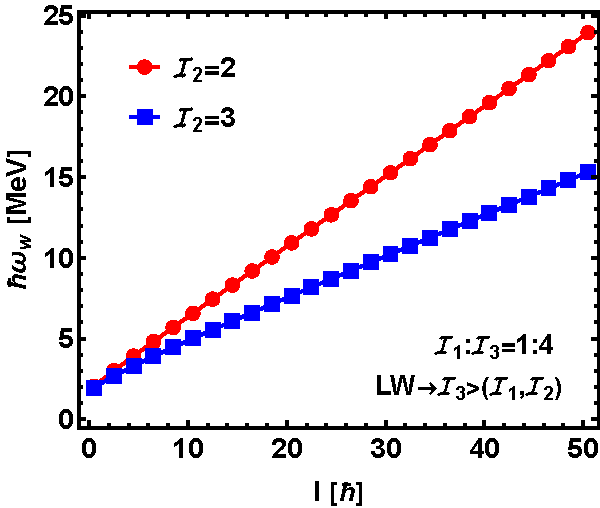
\includegraphics[width=0.49\textwidth]{Chapters/Figures/wobb_freq_oddA-LW.pdf}
    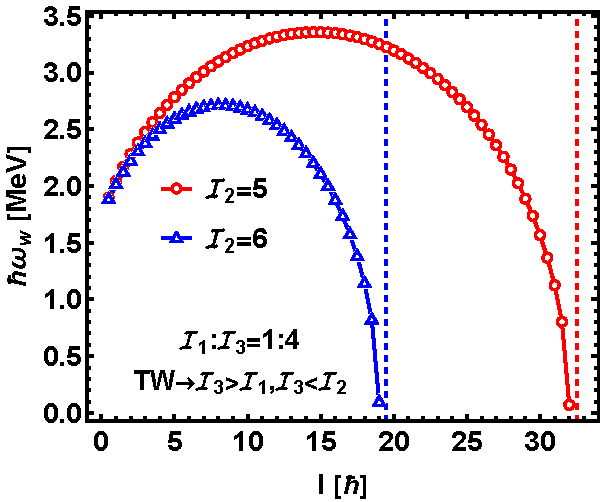
\includegraphics[width=0.49\textwidth]{Chapters/Figures/wobb_freq_oddA-TW.pdf}
    \caption{The wobbling frequency for an odd-$A$ nucleus, with the $\mathcal{Q}$'s a.m. $j=13/2$, coupled to the core $\mathscr{C}$. \textbf{Left:} The \emph{longitudinal wobbler} case with two sets of MOI, where only $\mathcal{I}_2$ differs. \textbf{Right:} The \emph{transverse wobbler} case with two sets of MOI, where only $\mathcal{I}_2$ is different. Note the vertical grid-lines in the right inset, signifying the critical angular momentum where the wobbling frequency reaches zero. The maximum value reached in the TW regime is given by Eq. \ref{wobb-freq-oddA-maxval}. The unit for MOI is $\hbar^2\text{MeV}^{-1}$.}
    \label{wobbling-freq-oddA}
\end{figure}

In the same manner as for the simple wobbler, a geometrical representation for the coupling schemes in the longitudinal and transverse wobbling motion can be made in order to get a grasp on the alignments between the quasi-particle and the triaxial ellipsoid. As such, Fig. \ref{wobbling-oddA-geometry} shows these representations. Besides these two wobbling regimes that emerge from FA approximation, two more wobbling modes can exist. Namely, for the \emph{yrast state} (that is the lowest energy state for a given value of angular momentum $I$, which can be regarded as a ground-state) and the \emph{excited state} of the odd particle itself. When the a.m. of the odd nucleon $\mathbf{j}_\mathcal{Q}$ starts to execute small precession around one of the principal axes of the triaxial core, then those excited states are viewed as \emph{signature partners} (since the de-alignment of the a.m. will cause the apparition of the favored and un-favored sequences, as described in Section \ref{section-ral-signature}). The yrast wobbling is simply regarded as a complete alignment of the odd-nucleon and core angular momenta with the $m$-axis, which is similar to the LW case except that there is no precessional motion for the angular momenta. These two particular cases are graphically represented in Fig. \ref{wobbling-geometry-YRAST-SPB}.
\begin{figure}
    \centering
    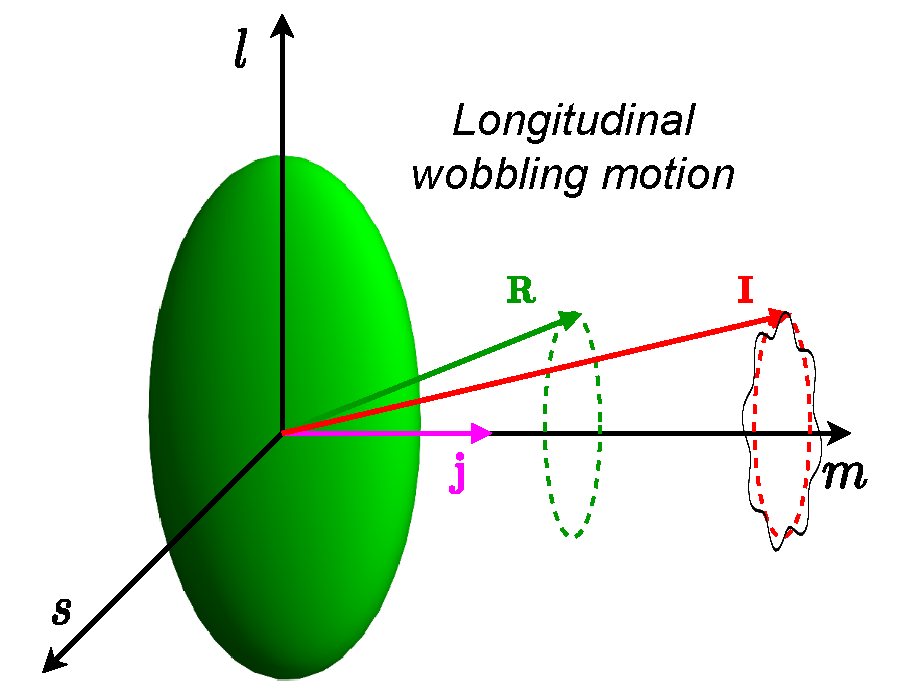
\includegraphics[width=0.49\textwidth]{Chapters/Figures/longitudinal_wobbler-schematic.pdf}
    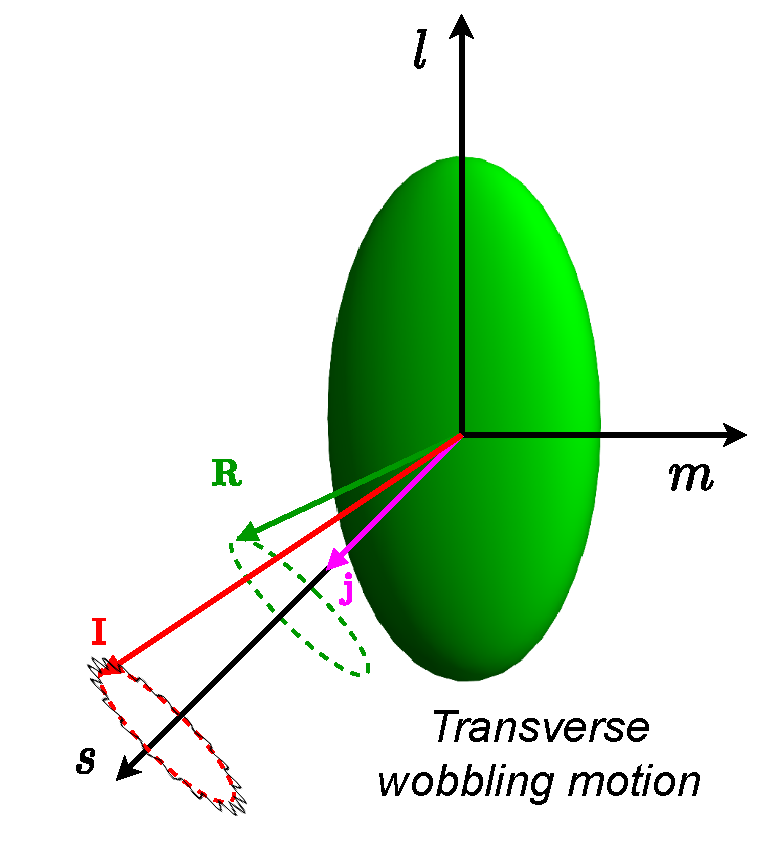
\includegraphics[width=0.49\textwidth]{Chapters/Figures/transverse_wobbler-schematic.pdf}
    \caption{Geometrical representation with the alignment scheme for a longitudinal wobbler and a transverse wobbler. The the a.m. vectors for the quasi-particle, the core, and the total system are represented by $\mathbf{j}_\mathcal{Q}$, $\mathbf{R}_\mathscr{C}$, and $\mathbf{I}$, respectively. Note that the precessional motion with oscillator-like behavior of $\mathbf{I}$ is illustrated with the encircled sine wave (black color). The resulting motion of the total a.m. will consist in a precessional cone that is properly depicted in Figs. \ref{advanced-quasiparticle-coupling-1}-\ref{advanced-quasiparticle-coupling-3}.}
    \label{wobbling-oddA-geometry}
\end{figure}
\begin{figure}
    \centering
    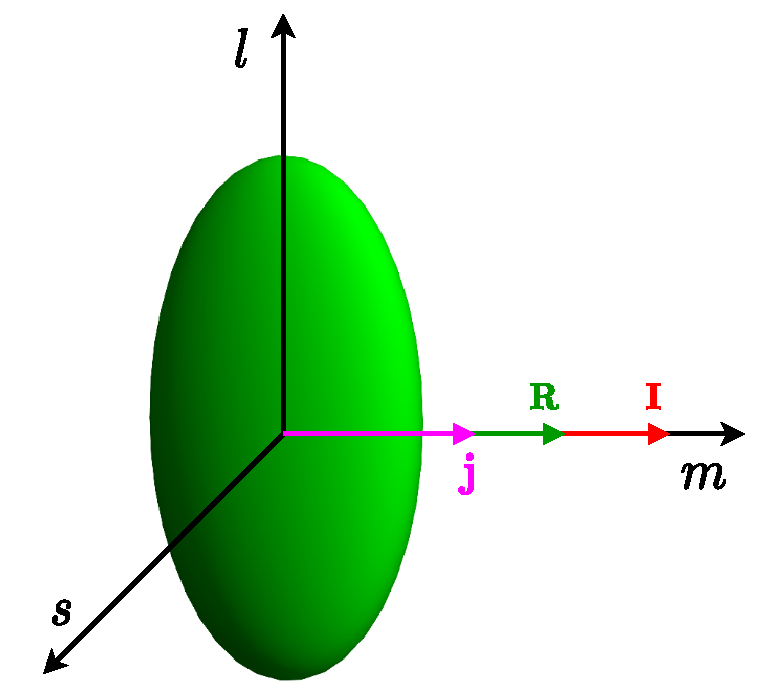
\includegraphics[width=0.49\textwidth]{Chapters/Figures/yrast_wobbler-schematic.pdf}
    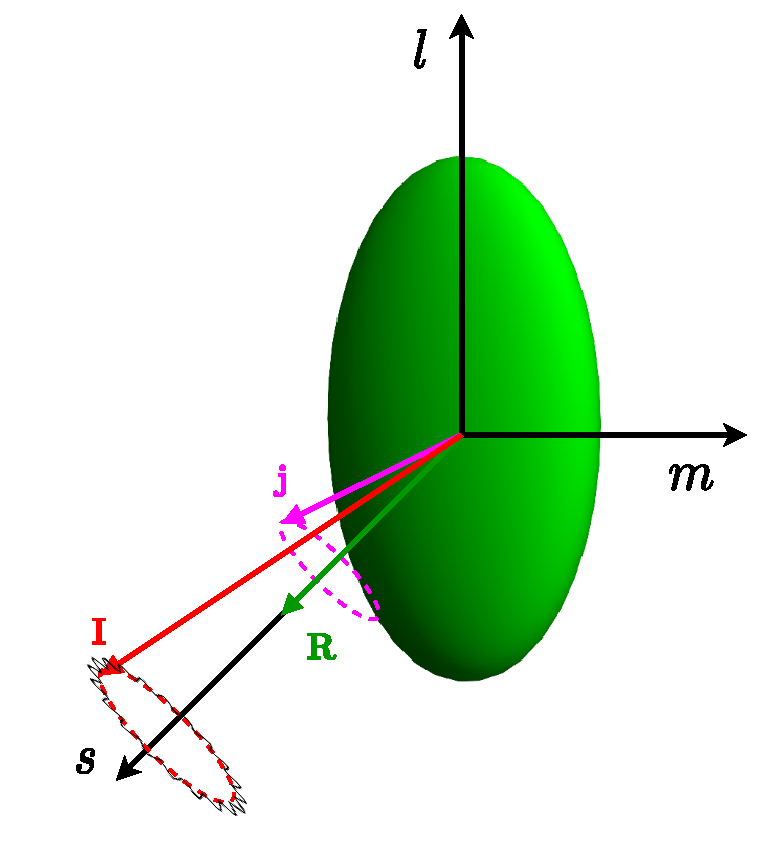
\includegraphics[width=0.49\textwidth]{Chapters/Figures/signaturePartner_wobbler-schematic.pdf}
    \caption{Geometrical representation with the alignment scheme for an yrast wobbling state and signature partner wobbling band. The the a.m. vectors for the quasi-particle, the core, and the total system are represented by by $\mathbf{j}_\mathcal{Q}$, $\mathbf{R}_\mathscr{C}$, and $\mathbf{I}$, respectively. Note that the precessional motion with oscillator-like behavior of $\mathbf{I}$ is illustrated with the encircled sine wave (black color). For the signature partner wobbling, the core's a.m. is aligned with one of the principal axes. The resulting motion of the total a.m. will consist in a precessional cone that is properly depicted in Figs. \ref{advanced-quasiparticle-coupling-1}-\ref{advanced-quasiparticle-coupling-3}.}
    \label{wobbling-geometry-YRAST-SPB}
\end{figure}

In this section, the collective motion specific to triaxial structures was treated for an odd-$A$ nucleus, starting from an initial rotor Hamiltonian, amended with a single-particle term. It was shown that based on the $\mathcal{Q}$+$\mathscr{C}$ coupling scheme, two scenarios might emerge, and the geometrical representation for both of them is illustrated in Fig. \ref{wobbling-oddA-geometry}. For transverse and longitudinal wobbling, some workflow diagrams were developed (see Figs. \ref{advanced-quasiparticle-coupling-1}-\ref{advanced-quasiparticle-coupling-3}) that explain how each behavior emerges based on $j$-shell filling and density overlap. Furthermore, the LW regime is characterized by an increase in wobbling energy with spin, while the opposite is true for TW regime. By keeping the quasi-particle's a.m. fixed along a principal axes, the expression for $\hat{H}$ was obtained via Eq. \ref{hamiltonian-qtr-FA} (in the Harmonic Approximation), which is quite close to the case of even-even nuclei (see Eq. \ref{general-rotor-ham-evenA}). The wobbling frequencies were also expressed (see Eqs. \ref{wobbling-frequency-odd-A-inertiaParams} - \ref{wobbling-frequency-odd-A-MOI}) and their behavior is analyzed with respect to spin (see Fig. \ref{wobbling-freq-oddA}). The reduced inertia factor $\mathscr{A}_3$ introduced in Eq. \ref{reduced-inertia-parameter-A3} is also studied w.r.t. the total spin $I$, and its evolution was shown in Fig. \ref{reduced-inertia-A3-figs}.

\section{Wobbling Nuclei - A Complete Catalog}

In this section, an inventory of all the known wobbling nuclei will be made. It is worth mentioning that there are ongoing debates regarding the experimental measurements and their `validity' for some of these isotopes, implying that wobbling phenomenon might not be present in some of them. Any existing conjecture will be mentioned where needed. For each wobbler, the band structure, the deformation parameters, and other important observations will be emphasized. Knowing the deformation parameters, one can also categorize the isotopes within regions of \emph{normal deformation} (ND structures) or \emph{strong deformation} (SD structure).

Although WM was predicted theoretically more than 50 years ago by Bohr and Mottelson \cite{bohr1998nuclear}, the first experimental observation of this collective mode has been confirmed in 2001. Moreover, the predictions were initially made for even-even nuclei, but the first nucleus in which wobbling was identified is the odd-$A$ $^{163}$Lu \cite{odegaard2001evidence}. The advance in technological equipment that allows high resolution/precision measurements has been very persistent over the last two decades, resulting in more and more successful investigations of the nucleonic matter at very high angular momentum ($I\approx 50\hbar$ or even $I\approx 80\hbar$). In the following subsections, the known wobblers will be categorized based on the atomic mass $A$, whereas a final diagram will be mapped at the end of this section. The mapping procedure is another useful feature of this current work, since it provides an easy and quick way of visualizing the progress towards the wobbling spectroscopy in the field of nuclear physics. This also constitutes the incipient phase for the development of an \emph{online digital register} with the current nuclei that will provide even more data.

\subsection{Wobbling around A=100}

In this region, recent measurements show that $^\mathbf{105}$\textbf{Pd} \cite{timar2019experimental} has two rotational bands built as wobbling excitations. The odd quasi-particle is a neutron from the $h_{11/2}$ orbital that is coupling to the even-even core. The $\mathcal{Q}+\mathscr{C}$ coupling in which the valence nucleon is a neutron represents a rare example across the nuclide chart. The even-even nucleus $^\mathbf{112}$\textbf{Ru} \cite{hamilton2010super} is also considered to have three wobbling bands (one yrast and two excited), indicating that from the three isotopes $^{108,110,112}$Ru, this one is the only one exhibiting a stable triaxial shape. Moreover, this isotope represents one of the few examples of collective excitations emerging from even-even nuclei. Additionally, some measurements on $^\mathbf{114}$\textbf{Pd} \cite{luo2013triaxial} (an isotone of the previous nucleus) show that the two bands with different signature ($\alpha=0$ and $\alpha=1$) have similar behavior with the ones from $^{112}$Ru (the excitation energies as function of angular momentum vary in the same fashion). However, the determination of mixing ratios and transition probabilities between levels was not possible, so the interpretation of these structures as wobbling bands cannot be fully ascertained \cite{lv2022experimental}. The behavior of the wobbling energy $E_\text{wob}$ as defined in Eq. \ref{eq-wobbling-energy-definition-oddA} is calculated for all the mentioned nuclei, using the available experimental data, and the results are shown in Fig. \ref{wobblers-exp-set1}.
\begin{figure}
    \centering
    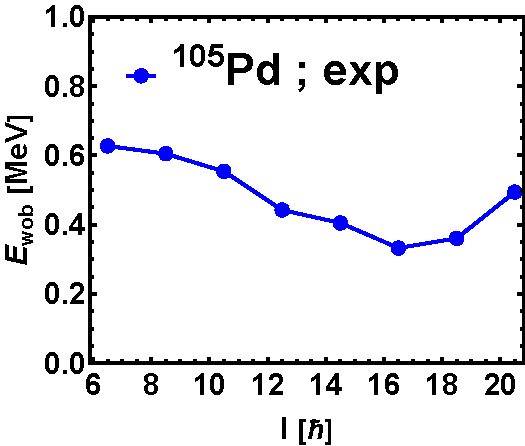
\includegraphics[width=0.32\textwidth]{Chapters/Figures/wobblers/105Pd.pdf}
    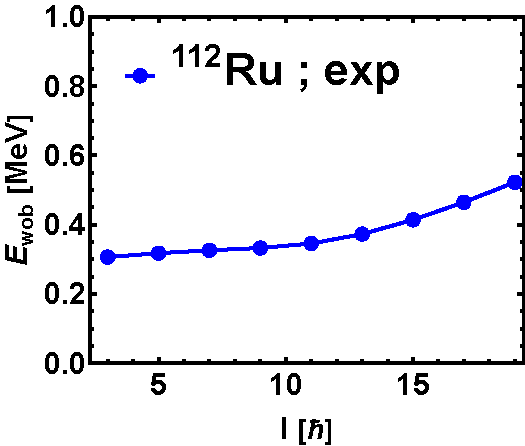
\includegraphics[width=0.32\textwidth]{Chapters/Figures/wobblers/112Ru.pdf}
    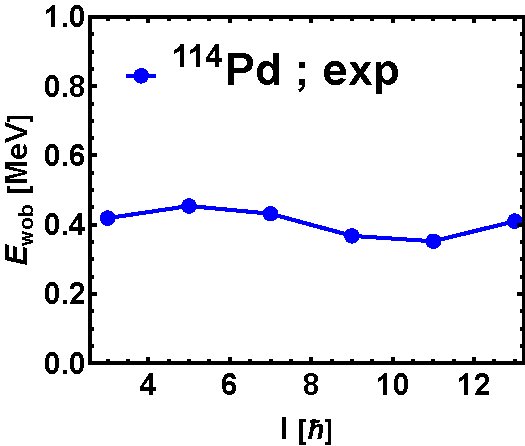
\includegraphics[width=0.32\textwidth]{Chapters/Figures/wobblers/114Pd.pdf}
    \caption{The experimental wobbling energy, defined through the Eq. \ref{eq-wobbling-energy-definition-oddA}, for nuclei within the $A\approx 100$ mass region. Data are taken from references cited in text for each isotope.}
    \label{wobblers-exp-set1}
\end{figure}

\subsection{Wobbling around A=130}

Chakraborty et al. \cite{chakraborty2020multiphonon} identified some wobbling bands in the odd-$A$ $^\mathbf{127}$\textbf{Xe} isotope. The collective states are built on the odd $\nu h_{11/2}$ nucleon configuration, leading to the apparition of four bands, two decoupled bands (i.e., favored $\alpha=-1/2$ and un-favored $\alpha=1/2$) with zero-phonon number, and two excited ($n_w=1,2$) wobbling bands. The wobbling energies (as defined in Eq. \ref{eq-wobbling-energy-definition-oddA}) are increasing with angular momentum, indicating that $^{127}$Xe behaves as a longitudinal wobbler. Another presumably longitudinal wobbler is the nucleus $^\mathbf{133}$\textbf{La} \cite{biswas2019longitudinal} with two wobbling bands $n_w=0$ and $n_w=1$ that exhibit enhanced $E2$ transition probabilities and mixing ratios (which are considered hallmarks of wobbling motion). The neighboring nucleus $^\mathbf{135}$\textbf{Pr} was also investigated, and three wobbling bands are reported (the yrast and $n_w=1$ bands in \cite{matta2017transverse} and $n_w=2$ in \cite{sensharma2019two}). The remarking feature is that the wobbling energies for this isotope are decreasing functions of spin, meaning that the TW regime prevails. The transition from LW to TW between $^{133}$La and its close neighbor $^{135}$Pr is a remarking feature of this elusive phenomenon. An insight into this change in motion will be discussed at the end of the section. Although there is inconclusive evidence regarding transition probabilities and mixing ratios \cite{ma1990competing,kaur2014high}, the yrast band from $^\mathbf{131}$\textbf{Ba} which is built on the $h_{11/2}$ neutron hole (i.e., $\mathcal{Q}_h$) can have an excited wobbling band, with negative parity spins ranging from $13/2$ to $29/2$ \cite{petrache_2018}. If precise measurements for the transition probabilities $B(E2)$ will show enhanced values, then indication of transverse wobbling will be decisive.

The isotope $^\mathbf{133}$\textbf{Ba} is another odd-mass nucleus in which three wobbling bands have been identified quite recently by Devi et al. \cite{devi2021observation}. Besides the excited $n_w=1$ and $n_w=2$, the yrast $n_w=0$ band has a signature partner band. All four bands have negative parity states. Devi et al. found out that the wobbling energies and the alignment behave quite similarly to $^{135}$Pr, concluding that this nucleus is a transverse wobbler. The remarking characteristic of this nucleus is that a hole-like particle $\mathcal{Q}_h$ couples to the core $\mathscr{C}$, stabilizing the total system to a deformed shape. Indeed, the odd $h_{11/2}$ neutron aligns itself with the long axis of the core, causing the TW regime to appear.

Within the last couple of years, a set of measurements brought light upon several even-even wobblers, although more precise measurements are required for ascribing triaxiality to this collective phenomenon with certainty. An example is the isotope that was studied in Section \ref{ba-130-numerical-calculations}, namely $^\mathbf{130}$\textbf{Ba} \cite{petrache2019diversity,chen2019transverse,wang2020two}. This nucleus exhibits wobbling via the coupling of two protons $\pi (h_{11/2})^2$ with the core $\mathscr{C}$. Such a coupling corresponds to a two-quasi-particle configuration in the nucleus, denoted here by 2-$\mathcal{Q}_h$ for holes and 2-$\mathcal{Q}_p$ for particles. Since the measurements of the transition probabilities show enhanced values and the wobbling energies decrease with spin, the isotope is regarded as a clear transverse wobbler. 

Petrache et al. also discovered wobbling motion within some nuclei that were heavily studied in terms of chirality (i.e., the Nd and Ce isotopes). In their research, it was found that $^\mathbf{134}$\textbf{Ce} has two `sets' of wobbling bands \cite{petrache2016transverse}. The first one is based on a 2-$\mathcal{Q}_h$ configuration with two neutron holes $\nu (h_{11/2})^2$ which align with the long axis, leading to a $n_w=0$ and $n_w=1$ structure (here the exponent signifies the number of holes relative to the notation $\mathcal{Q}_h$, and it is equivalent to the alternative notation $\nu(h_{11/2})^{-2}$ used for example in \cite{petrache2012tilted,lv2018evolution,chen2021microscopic}) that possesses negative triaxiality (that is $\gamma<0$). Similarly, two more bands emerge (zero- and one-phonon) from the coupling of the same 2-$\mathcal{Q}_h$ with the core, but their a.m. is aligned along the short axis of $\mathscr{C}$ and the triaxiality parameter $\gamma$ becomes positive. Both sets behave as transverse wobblers, but the latter set has a higher quadrupole deformation. In the same work \cite{petrache2016transverse}, the isotope $\mathbf{^{136}}$\textbf{Nd} has been confirmed as a TW. Remarking the fact that this nucleus also has two sets of bands. The first set (zero- and one-phonon wobbling bands) is built on the same neutron holes, where $\mathbf{j}_{\mathcal{Q}_h}$ aligns with the long axis and it brings the entire system to a negative triaxiality and low deformation. The second set has three bands (one yrast and two excited) that are built on two 2-$\mathcal{Q}_p$ (i.e., the $\pi(h_{11/2})^2$ protons), which align their a.m. with the short axis and drive the entire system to a larger deformation and positive $\gamma$.

Lastly, the isotope $^\mathbf{138}$\textbf{Nd} was investigated by Petrache et al. \cite{petrache2012tilted}, and some remarks about a possible wobbling behavior in the measured spectra were made. There is one excited band (labelled $L7$) that decays to the yrast band ($L6$), however, the configuration of the wobbling band is different than the yrast partner. Namely, the $L7$ band is built on a 2-$\mathcal{Q}_h$ neutron pair $\nu (h_{11/2})^2$ which aligns with the long axis (due to the hole character). For the yrast band, the configuration was determined to be more complex: a $g_{9/2}$ proton coupled to a $\nu (h_{11/2})^2$ neutron pair and one more additional neutron in the $g_{7/2}$ orbital, making thus an `overall' $2\mathcal{Q}_p\otimes2\mathcal{Q}_h$ configuration.

The behavior of the wobbling energy $E_\text{wob}$ as defined in Eq. \ref{eq-wobbling-energy-definition-oddA} is calculated for all the mentioned nuclei, and the results are shown in Fig. \ref{wobblers-exp-set2}. Exception is the isotope $^{138}$Nd, where a plot showing both the $n_w=0$ and $n_w=1$ bands with the absolute values for energy is used instead. For $^{135}$Pr, the transition from a TW regime to LW which was identified in \cite{sensharma2019two} is marked by two colored regions (green for TW and red for LW).
% \begin{figure}[H]
\begin{figure}
    \centering
    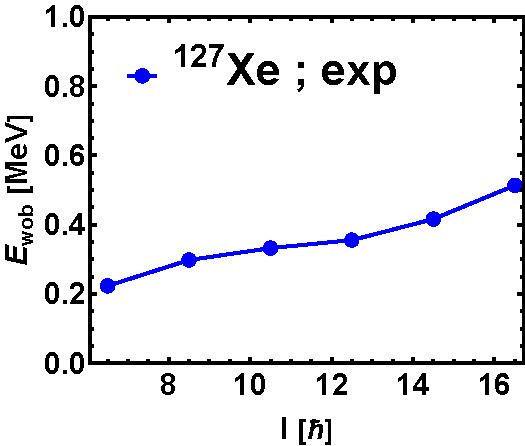
\includegraphics[width=0.32\textwidth]{Chapters/Figures/wobblers/127Xe.pdf}
    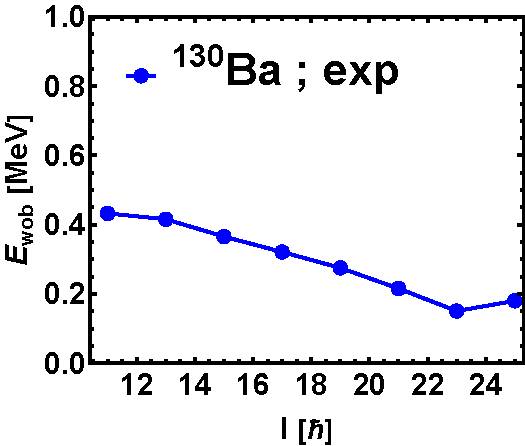
\includegraphics[width=0.32\textwidth]{Chapters/Figures/wobblers/130Ba.pdf}
    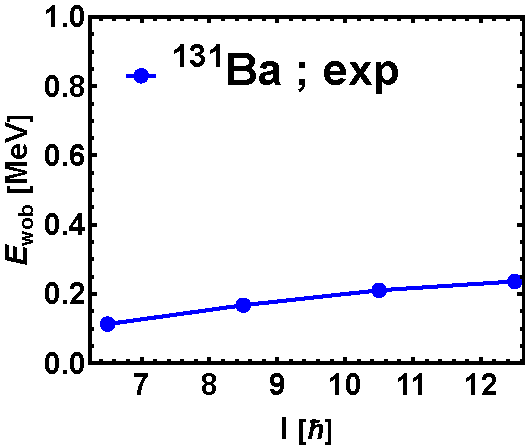
\includegraphics[width=0.32\textwidth]{Chapters/Figures/wobblers/131Ba.pdf}
    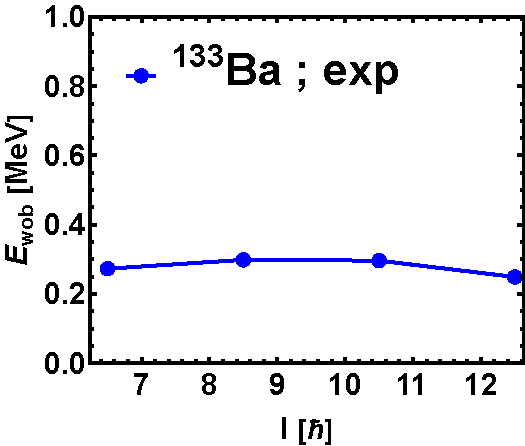
\includegraphics[width=0.32\textwidth]{Chapters/Figures/wobblers/133Ba.pdf}
    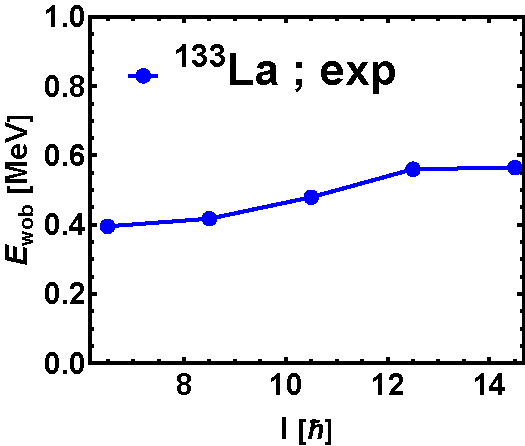
\includegraphics[width=0.32\textwidth]{Chapters/Figures/wobblers/133La.pdf}
    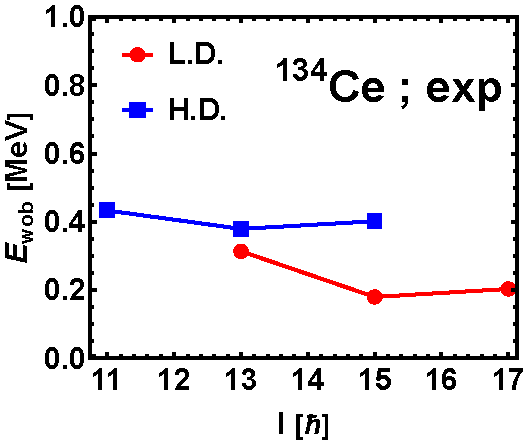
\includegraphics[width=0.32\textwidth]{Chapters/Figures/wobblers/134Ce-joint.pdf}
    % 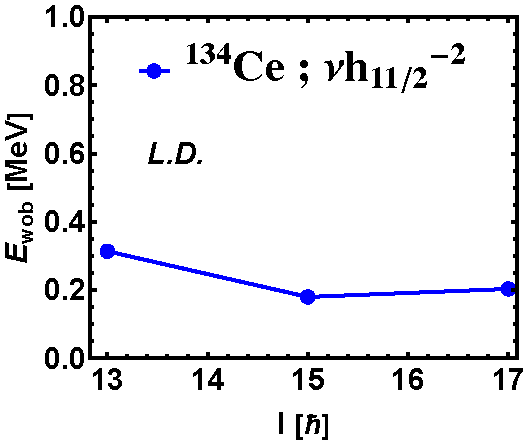
\includegraphics[width=0.32\textwidth]{Chapters/Figures/wobblers/134Ce-1.pdf}
    % 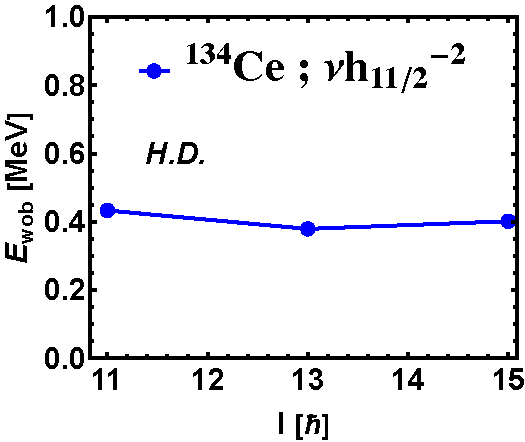
\includegraphics[width=0.32\textwidth]{Chapters/Figures/wobblers/134Ce-2.pdf}
    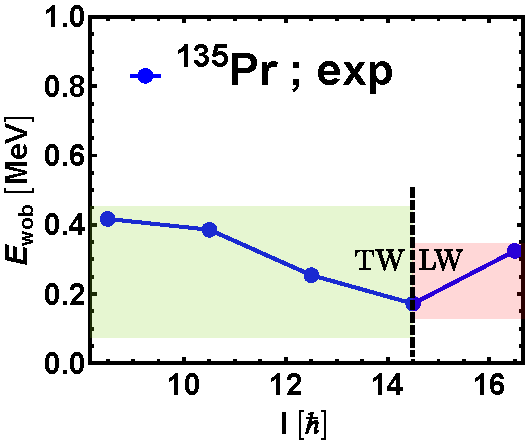
\includegraphics[width=0.32\textwidth]{Chapters/Figures/wobblers/135Pr-edited.pdf}
    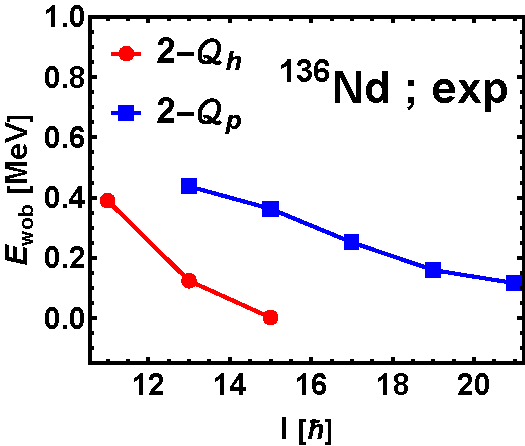
\includegraphics[width=0.32\textwidth]{Chapters/Figures/wobblers/136Nd-joint.pdf}
    % 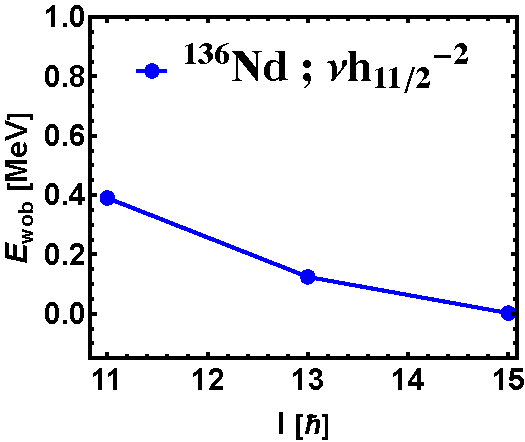
\includegraphics[width=0.32\textwidth]{Chapters/Figures/wobblers/136Nd-1.pdf}
    % 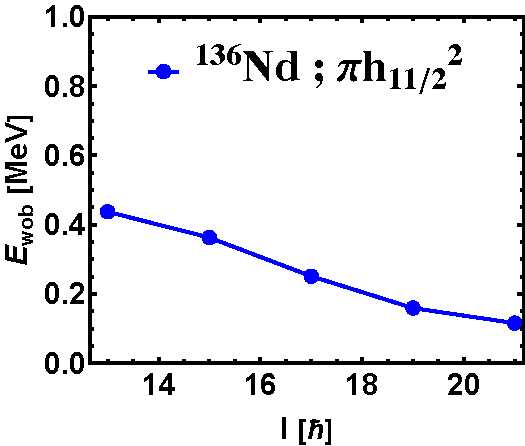
\includegraphics[width=0.32\textwidth]{Chapters/Figures/wobblers/136Nd-2.pdf}
    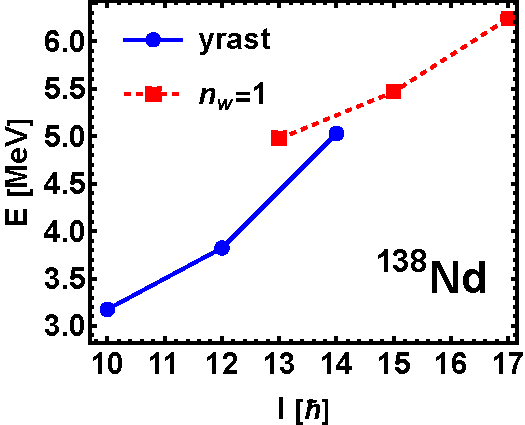
\includegraphics[width=0.32\textwidth]{Chapters/Figures/wobblers/138Nd.pdf}
    \caption{The experimental wobbling energy, defined through the Eq. \ref{eq-wobbling-energy-definition-oddA}, for nuclei within the $A\approx 130$ mass region. For $^{134}$Ce, the two abbreviations denote the bands with lower deformation (L.D.) and higher deformation (H.D.), respectively. For $^{136}$Nd, the two configurations are represented by 2-$\mathcal{Q}_h$ for the neutron holes and 2-$\mathcal{Q}_p$ for the protons that couple with the core. See text for more details.}
    \label{wobblers-exp-set2}
\end{figure}

\subsection{Wobbling around A=160}

A highly-aligned $\mathcal{Q}$ will favor a specific triaxial shape \cite{hamamoto1983intrinsic} given by the $j$-orbital in which it belongs to. Moreover, the degree of shell filling will dictate a particular value for the triaxiality parameter $\gamma$. In turns out that for this proton, the favored triaxiality is around $\gamma=20^\circ$, meaning that PES calculations on strongly deformed triaxial structure will show stable minima around that $\gamma$-value. The wobbling excitations appear since only a small rotational energy is needed for building excited levels above the yrast line \cite{hamamoto2016interplay}.

Experimentally, this is the \emph{richest} region within the chart of nuclides characterized that by wobbling motion. As mentioned at the start of the section, the first ever nucleus in which this phenomenon has been observed was $^\mathbf{163}$\textbf{Lu} \cite{odegaard2001evidence}. With a huge infrastructure available at the Euroball detector \cite{simpson1997euroball}, two \emph{triaxial strongly deformed} bands (TSD1 and TSD2) with similar properties were measured. Both bands were built on the configuration of a $\mathcal{Q}_p$ proton which belongs to the $i_{13/2}$ orbital. In fact, along the $A\approx 160$ region, this \emph{intruder} will cause most of the triaxial structures to become highly-deformed and stable. One year later, a second excited wobbling band (TSD3) was confirmed \cite{jensen2002evidence}, and in a recent work by Raduta et al. (i.e., the current team) \cite{raduta2017semiclassical,raduta2020towards} the third excited phonon band (TSD4) was ascribed to the wobbling character. The measurements indicate large quadrupole values, positive triaxiality, and enhanced quadrupole transitions. Furthermore, quantities such as alignment, dynamic moment of inertia, and excitation energies relative to a reference show similarities across each of the four bands, with magnitudes that are higher than other neighboring (coexisting) normally-deformed structures \cite{jensen2004coexisting}. This is a clear indicator that stable triaxial structures exist in $^{163}$Lu. After this discovery, a large number of wobbling bands, appearing at large deformation parameters were identified in $^\mathbf{161}$\textbf{Lu} \cite{bringel2005evidence} (one excited wobbling band), $^\mathbf{165}$\textbf{Lu} \cite{schonwasser2003one} (two excited), $^\mathbf{167}$\textbf{Lu} \cite{amro2003wobbling} (one excited), and $^\mathbf{167}$\textbf{Ta} \cite{hartley2009wobbling} (one excited).

It is worth mentioning that the isotopes in this particular region have large spins, meaning that they are also rapidly rotating. When fast rotation occurs, both the core as well as the particle's a.m. will align with the intermediate axis, meaning that these wobblers behave as longitudinal wobblers. However, qualitatively, the wobbling energies have a decreasing trend with spin $I$, showing a transverse-like character. Keep in mind that for large angular momentum values, the TW/LW description becomes unstable, since that approximation requires low spins. For the high-spin region, the wobbling mechanism is explained through a `top-on-top' model \cite{hamamoto2002wobbling,tanabe2006algebraic} (analogy with the classical asymmetric top). The behavior of the wobbling energy $E_\text{wob}$ as defined in Eq. \ref{eq-wobbling-energy-definition-oddA} is calculated for all the mentioned nuclei, using the available experimental data, and the results are shown in Fig. \ref{wobblers-exp-set3}.
\begin{figure}
    \centering
    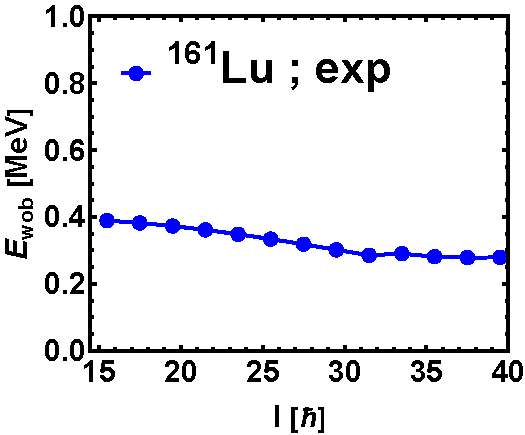
\includegraphics[width=0.32\textwidth]{Chapters/Figures/wobblers/161Lu.pdf}
    \includegraphics[width=0.32\textwidth]{Chapters/Figures/wobblers/163Lu.pdf}
    \includegraphics[width=0.32\textwidth]{Chapters/Figures/wobblers/165Lu.pdf}
    \includegraphics[width=0.32\textwidth]{Chapters/Figures/wobblers/167Lu.pdf}
    \includegraphics[width=0.32\textwidth]{Chapters/Figures/wobblers/167Ta.pdf}
    \caption{The experimental wobbling energy, defined through the Eq. \ref{eq-wobbling-energy-definition-oddA}, for nuclei within the $A\approx 160$ mass region. Data are taken from references cited in text for each isotope.}
    \label{wobblers-exp-set3}
\end{figure}

\subsection{Wobbling around A=180}

A set of new measurements show some wobbling structures in the heavy-nuclei region. Namely, the isotopes $^\mathbf{183}$\textbf{Au} \cite{nandi2020first} and $^\mathbf{187}$\textbf{Au} \cite{sensharma2020longitudinal,sensharma2021wobbling}. In the former, two wobbling bands were identified, one built on a positive parity proton $i_{13/2}$ and one built on a negative parity proton $h_{9/2}$. The remarking feature of this nucleus is that even though both protons align perpendicular to the intermediate axis (typical to a TW regime) the wobbling energies exhibit a decrease (the $n_w=1$ band built on the positive parity proton). As a matter of fact, Nandi et al. speculate that these states represent the initial increasing part of the wobbling energy as function of spin for a TW. Remember that the wobbling frequency of a TW system (Eqs. \ref{wobbling-frequency-odd-A-inertiaParams} - \ref{wobbling-frequency-odd-A-MOI}) has an increasing part in the low-spin region, and only after a critical $\mathscr{I}$ value (i.e., Eq. \ref{wobb-freq-oddA-maxval}) the frequency starts to decrease (according to Fig. \ref{wobbling-freq-oddA}). Moreover, an interesting remark is raised, suggesting that the increasing/decreasing trend for wobbling energies must not be considered as the sole indicator for LW/TW regime (this discussion is also emphasized in a recent work done by Poenaru and Raduta \cite{poenaru2021extensive1,poenaru2021extensive2}). The $^{187}$Au nucleus exhibits longitudinal wobbling motion, having one yrast and one excited band. Both bands are built on the configuration of a proton from $h_{9/2}$ $j$-orbital, located at the middle of the shell, suggesting a LW behavior (since the $\mathcal{Q}$ will align its a.m. along the $m$-axis of the core). 

The behavior of the wobbling energy $E_\text{wob}$ as defined in Eq. \ref{eq-wobbling-energy-definition-oddA} is calculated for the two nuclei in $A\approx 180$ region, using the available experimental data, and the results are shown in Fig. \ref{wobblers-exp-set4}.
\begin{figure}
    \centering
    \includegraphics[width=0.33\textwidth]{Chapters/Figures/wobblers/183Au_2-edited.pdf}
    \includegraphics[width=0.32\textwidth]{Chapters/Figures/wobblers/183Au_1.pdf}
    \includegraphics[width=0.32\textwidth]{Chapters/Figures/wobblers/187Au.pdf}
    \caption{The experimental wobbling energy, defined through the Eq. \ref{eq-wobbling-energy-definition-oddA}, for nuclei within the $A\approx 180$ mass region. Data are taken from references cited in text for each isotope. Note that for $^{183}$Au, there are two configurations which cause wobbling motion, namely, the protons $\pi i_{13/2}$ (positive parity) and $\pi h_{9/2}$ (negative parity). Nandi et al. \cite{nandi2020first} suspect that the behavior of the former band is justified by a transverse-like wobbling frequency which increases up to a certain spin before it stats to decrease. This is illustrated via the small inset inside the first figure, where the wobbling frequencies for a TW nucleus are sketched (according to Eq. \ref{wobbling-frequency-odd-A-MOI} and Fig. \ref{wobbling-freq-oddA}).}
    \label{wobblers-exp-set4}
\end{figure}

\subsubsection*{Evidence Against Wobbling Motion}

Recently, the interpretation of nuclei around the $A \approx 130$ as wobblers was questioned by several teams \cite{nomura2021examining,nomura2022questioning,lv2022evidence,guo2020risk}. This is due to the fact that in the low-spin region, the wobbling mode (which consists of phonon-like excitations) will compete with single-particle excitations. As such, a clear difference must be made between the two modes. Experimentally, it was shown that signatures for wobbling excitations are the enhanced quadrupole moments and rather large mixing ratios $\delta(E2/M1)$ (which indicate a competition between E2 or M1 transitions within states belonging to adjacent collective bands). However, the data for $A\approx 100-130$ show rather small quadrupole deformations and a $\gamma$-soft character of the deformed potential, unlike the heavier isotopes at the $A \approx 160$ mass region. The obtained transition probabilities connecting the states between bands are obtained from experimental methods which are beyond the scope of this work, but for reference one can check \cite{lv2022evidence}. Consequently, it is of crucial importance to have precise determination of the experimental quantities such as E2/M1 mixing ratios between bands, in order to be certain of the actual nature of the studied isotopes.

For collective excitations, the dominant E2 character of the linking transitions between the $n_w=1$ and yrast bands must have mixing ratios larger than unity. Keep in mind that the mixing ratio for a particular $\Delta I=1$ transition is typically defined as \cite{krane1970determination,nomura2021examining}:
\begin{align}
    \delta=c\cdot E_\gamma\frac{\bra{I_f}|\mathcal{M}(E2)|\ket{I_i}}{\bra{I_f}|\mathcal{M}(M1)|\ket{I_i}}, 
\end{align}
with $E_\gamma=E(I_i)-E(I_f)$ and the reduced matrix elements $\mathcal{M}(E2)$, $\mathcal{M}(M1)$ corresponding to the electric quadrupole and magnetic dipole transitions, respectively. As mentioned, this mixing ratio is expected to be $\delta >1$ for wobbling excitations. Apparently, after new measurements performed on the the discovered wobbling bands in the low spin region for $^{105}$Pd, $^{135}$Pr, $^{133}$La, $^{133}$Ba, $^{135}$Pr might have mixing ratios $\delta<1$, meaning that the magnetic transitions are more enhanced. The magnetic dominance would rule out wobbling mode, thus raising the question wether the wobbling phenomenon is indeed present or not. These newly conducted measurements lead to mixing ratios less than one, which is in favor of an entire re-evaluation, in particular for $^{133}$La \cite{hua2020comment} and $^{135}$Pr \cite{guo2021comment,lv2022evidence}.

Besides the wobbling motion, other collective phenomena can arise in the yrast and excited bands of triaxial nuclei. One example is the so-called Tilted-Axis-Precession (TiP) \cite{lawrie2020tilted}, which is a very recent description for the rotational properties of non-axial nuclei. Lawrie et al. showed that tilted precession behaves quite similarly to wobbling motion, and at low spins there can be a `competition' between the two. Remarking the fact that TiP effect implies a precession of the total angular momentum which does not require the quantization of the energy in terms of vibrational phonons. Moreover, the precession does not have to be around one of the principal axes of the triaxial ellipsoid, so it can precesses around a tilted axis. This interesting process was in fact used to describe the motion in $^{135}$Nd \cite{lv2021tilted} and it seems to be drawing a lot of attention lately.

\subsubsection*{The Transition Between Wobbling Regimes}

The already discussed isotopes $^{133}$La and $^{135}$Pr show an interesting phenomenon, where the former exhibits an increasing energy, while the latter (with only two extra nucleons) reveals a decreasing trend. This rather `abrupt' change in the $\mathcal{Q}+\mathscr{C}$ coupling, (i.e., parallel alignment of $\mathcal{Q}$ with the core in the first case, and perpendicular alignment in the second) was explained by Biswas et al. \cite{biswas2019longitudinal}. Indeed, in both nuclei the $\mathcal{Q}_p$ ($h_{11/2}$ proton) is expected to align with the $s$-axis, such that the two isotones must exhibit transverse wobbling. But the situation can be understood in the following way: the $\mathcal{Q}_p$ in $^{135}$Pr aligns its a.m. with the short axis of the triaxial core and since the $m$-axis has the largest MOI, TW will arise. However, for $^{133}$La, besides the $h_{11/2}$ proton, an extra pair of protons (positive-parity) will align gradually with the $s$-axis of the triaxial density distribution. It is this additional alignment that increases the effective MOI of the short axis, which achieves a higher magnitude than the one along the $m$-axis. This re-arrangement will finally result in the LW behavior of the isotope.

The LW/TW behavior within the two nuclei can also be understood in terms of angular momentum behavior w.r.t. the rotational frequency (i.e., the backbending curves, such as the ones presented in Figs. \ref{fig-hfNuclei-mois} - \ref{fig-ErYbnuclei-mois}). For $^{133}$La, there is a rather constant and gradual increase in spin with the rotational frequency. On the other hand, $^{135}$Pr shows a strong backbend with increasing spin (although rather late). Additionally, both nuclei show rotation around the short axis close to the yrast line (since the proton will align its a.m. with that axis). For $^{135}$Pr, $\mathcal{I}_s$ is smaller than $\mathcal{I}_m$, and with increasing spin it becomes convenient to add more and more collective angular momentum on the $m$-axis. Consequently, the wobbling frequency will start to decrease with increasing spin and so does the final wobbling energy. Such a mechanism clearly leads to transverse regime. At the same time, the ratio $\mathcal{I}_s/\mathcal{I}_m$ is closer to $1$ for $^{133}$La, meaning that the medium axis is no longer preferred by the collective rotation, and the $s$-axis will start to gain more and more angular momentum. The increase of collective a.m. along the short axis causes the wobbling frequency to increase with spin, which is specific to the longitudinal character. The evolution with rotational frequency of the total angular momentum in both nuclei can be seen in Fig. \ref{spin-vs-rotationalFreq-133-135}. Notice the gradual increase of the yrast band for $^{133}$La vs. the sharp backbend present in $^{135}$Pr.
\begin{figure}
    \begin{center}
        \includegraphics[width=0.49\textwidth]{Chapters/Figures/133La_wob-edited.pdf}
        \includegraphics[width=0.49\textwidth]{Chapters/Figures/135Pr_wob-edited.pdf}
        \caption{The angular momentum evolution with respect to the (experimental) rotational frequency $\omega_\text{rot}$ for $^{133}$La (\textbf{left}) and $^{135}$Pr (\textbf{right}). The backbending region for the latter nucleus is illustrated within the colored sector. Since the $s$-axis MOI is smaller, more and more collective a.m. will be added to this axis, causing a decrease in the wobbling frequency (TW). The dotted magenta line represents the angular momentum value for the odd proton.}
        \label{spin-vs-rotationalFreq-133-135}
    \end{center}
\end{figure}

\subsection{Wobbling - Experimental Chart}

All the currently known wobblers where there is enough (or at least some tentative) experimental data that indicate wobbling were grouped in the four main regions, namely, $A\approx 100, 130, 160$ and $180$, respectively. Following up, a chart will be constructed, showing all wobblers with some important values such as the quadrupole deformation parameter, triaxiality parameter, and wobbling regime. This is an inedited representation of the nuclides and the first \emph{unified depiction} of wobbling nuclei in terms of their deformation parameters. The scheme can be seen in Fig. \ref{wobbling-diagram-chart}, however, the reader should firstly refer to Fig. \ref{wobbling-diagrams-legend} for explanation of an individual element within the chart.
\begin{figure}
    \centering
    \includegraphics[width=0.99\textwidth]{Chapters/Figures/wobblers-chart-legend.pdf}
    \caption{Example that describes each relevant parameter of a single nucleus from the wobbling chart shown in Fig. \ref{wobbling-diagram-chart}. This particular `legend' belongs to the $^{187}$Au isotope.}
    \label{wobbling-diagrams-legend}
\end{figure}
\begin{figure}
    \centering
    \includegraphics[width=0.97\textwidth]{Chapters/Figures/wobblers-chart.pdf}
    \caption{Unified chart showing the currently known wobblers. See Fig. \ref{wobbling-diagrams-legend} for legend. \emph{Strong deformation} is marked with red color for $\beta_2$.}
    \label{wobbling-diagram-chart}
\end{figure}

\section{Concluding Remarks}

Concluding this section and chapter, several important discussions were pointed out. Firstly, the formalism for wobbling motion in even-even nuclei was described, obtaining the energy spectrum and the wobbling frequency for a simple triaxial rotor (recall Eq. \ref{eq-wobbling-energy-evenA} and Eq. \ref{wobbling-frequency-even-A}). The geometrical representation of the angular momentum components in terms of the polar angles $(\theta,\varphi)$ was also realized for a given value of $I$ (see Fig. \ref{figs-angular-momentum-components-polar}). The Harmonic Approximation (HA) was tested for a known wobbler, i.e., the $^{130}$Ba isotope. Results concerning the excitation energies, quadrupole moments, and transition probabilities were evaluated and compared with the available experimental data. The agreement with the experimental data is quite well and this represents a new and original set of results that are presented in the current research. The next step consisted in the analysis of an odd-$A$ triaxial nucleus within the Quasi-Particle Triaxial Rotor model (QTR), whose model Hamiltonian was given by Eq. \ref{oddA-QTR-general-hamiltonian}. At low spins two possible wobbling motions were portrayed, namely the transverse and longitudinal wobbling. The difference between the two was explained in terms of particle-rotor coupling. 

Additionally, three workflow diagrams were illustrated (see Figs. \ref{advanced-quasiparticle-coupling-1} - \ref{advanced-quasiparticle-coupling-3}) with the aim of understanding how the different alignments of the odd quasi-particle ($\mathcal{Q}$) with the triaxial core ($\mathscr{C}$) are realized in terms of their density distribution overlap. A wobbling frequency in the odd-$A$ case was also obtained (Eq. \ref{wobbling-frequency-odd-A-MOI} through a similar harmonic approximation, and its behavior with angular momentum was quantitatively described for both wobbling regimes (see Fig. \ref{reduced-inertia-A3-figs}). Another set of geometrical representations were made for the wobbling modes which can occur in nuclei (see Figs. \ref{wobbling-geometry-YRAST-SPB}, \ref{simple-wobbler-geometrical-schematic}, and \ref{wobbling-oddA-geometry}) showing how the precession of each individual vector (i.e., core $\mathbf{R}_\mathscr{C}$, quasi-particle $\mathbf{j}_\mathcal{Q}$ and total $\mathbf{I}$) behaves relative to the entire ellipsoid. Lastly, an inventory with all the known wobbling nuclei was made, for different mass regions. Deformation parameters, wobbling bands, and wobbling characters were pointed out per each nucleus in a unified diagram (Fig. \ref{wobbling-diagram-chart}), which is a first within literature.

With the concept of wobbling motion fully explained from a theoretical standpoint, but also applied to specific numerical cases, one can get into the next step, which is the main part of this work. Namely, the description of wobbling motion in odd-$A$ nuclei will be studied in detail using a formalism based on a Particle-Rotor Model. Analytical results for the relevant quantities will be given, and important observations will be discussed when necessary.